%definira klasu dokumenta 
\documentclass[12pt]{report} 

%prostor izmedu naredbi \documentclass i \begin{document} se zove uvod. U njemu se nalaze naredbe koje se odnose na cijeli dokument

%osnovni LaTex ne može riješiti sve probleme, pa se koriste različiti paketi koji olakšavaju izradu željenog dokumenta
\usepackage[croatian]{babel} 
\usepackage{amssymb}
\usepackage{amsmath}
\usepackage{txfonts}
\usepackage{mathdots}
\usepackage{titlesec}
\usepackage{array}
\usepackage{lastpage}
\usepackage{etoolbox}
\usepackage{longtable, tabu}
\usepackage{color, colortbl}
\usepackage{adjustbox}
\usepackage{geometry}
\usepackage[classicReIm]{kpfonts}
\usepackage{hyperref}
\usepackage{fancyhdr}

\usepackage{float}
\usepackage{setspace}
\restylefloat{table}


\patchcmd{\chapter}{\thispagestyle{plain}}{\thispagestyle{fancy}}{}{} %redefiniranje stila stranice u paketu fancyhdr

%oblik naslova poglavlja
\titleformat{\chapter}{\normalfont\huge\bfseries}{\thechapter.}{20pt}{\Huge}
\titlespacing{\chapter}{0pt}{0pt}{40pt}


\linespread{1.3} %razmak između redaka

\geometry{a4paper, left=1in, top=1in,}  %oblik stranice

\hypersetup{ colorlinks, citecolor=black, filecolor=black, linkcolor=black,	urlcolor=black }   %izgled poveznice


%prored smanjen između redaka u nabrajanjima i popisima
\newenvironment{packed_enum}{
	\begin{enumerate}
		\setlength{\itemsep}{0pt}
		\setlength{\parskip}{0pt}
		\setlength{\parsep}{0pt}
	}{\end{enumerate}}

\newenvironment{packed_item}{
	\begin{itemize}
		\setlength{\itemsep}{0pt}
		\setlength{\parskip}{0pt}
		\setlength{\parsep}{0pt}
	}{\end{itemize}}


%boja za privatni i udaljeni kljuc u tablicama
\definecolor{LightBlue}{rgb}{0.9,0.9,1}
\definecolor{LightGreen}{rgb}{0.9,1,0.9}


%podesavanje zaglavlja i podnožja

\pagestyle{fancy}
\lhead{Programsko inženjerstvo}
\rhead{Online tečajevi}
\lfoot{JamesBondi}
\cfoot{stranica \thepage/\pageref{LastPage}}
\rfoot{\today}
\renewcommand{\headrulewidth}{0.2pt}
\renewcommand{\footrulewidth}{0.2pt}


\begin{document} 
	
	
	
	\begin{titlepage}
		\begin{center}
			\vspace*{\stretch{1.0}} %u kombinaciji s ostalim \vspace naredbama definira razmak između redaka teksta
			\LARGE Programsko inženjerstvo\\
			\large Ak. god. 2020./2021.\\
			
			\vspace*{\stretch{3.0}}
			
			\huge Online tečajevi\\
			\Large Dokumentacija, Rev. 1\\
			
			\vspace*{\stretch{12.0}}
			\normalsize
			Grupa: JamesBondi\\
			Voditelj: Marin Fabijanić\\
			
			
			\vspace*{\stretch{1.0}}
			Datum predaje: {13.11.2020.}\\
	
			\vspace*{\stretch{4.0}}
			
			Nastavnik: Nikolina Frid\\
		
		\end{center}

	
	\end{titlepage}

	
	\tableofcontents

	\chapter{Dnevnik promjena dokumentacije}
	
				
		
		\begin{longtabu} to \textwidth {|X[2, l]|X[13, l]|X[3, l]|X[3, l]|}
			\hline \multicolumn{1}{|l|}{\textbf{Rev.}}	& \multicolumn{1}{l|}{\textbf{Opis promjene/dodatka}} & \multicolumn{1}{|l|}{\textbf{Autori}} & \multicolumn{1}{l|}{\textbf{Datum}} \\[3pt] \hline
			\endfirsthead
			
			\hline \multicolumn{1}{|l|}{\textbf{Rev.}}	& \multicolumn{1}{l|}{\textbf{Opis promjene/dodatka}} & \multicolumn{1}{|l|}{\textbf{Autori}} & \multicolumn{1}{l|}{\textbf{Datum}} \\[3pt] \hline
			\endhead
			
			\hline 
			\endlastfoot
			
			0.1 & Napravljen predložak	& Sokolić & 16.10.2020. 		\\[3pt] \hline 
			0.2	& Dodan opis projektnog zadatka & Gojević &  20.10.2020.	\\[3pt] \hline 
			0.3 & Dodan prvi dio opisa obrazaca uporabe & Gojević & 23.10.2020. \\[3pt] \hline 
			0.3.1 & Dodani svi opisi obrazaca uporabe & Gojević & 24.10.2020. \\[3pt] \hline 
			0.3.2 & Nadopunjen opis projektnog zadatka & Sokolić & 24.10.2020. \\[3pt] \hline
			0.4 & Dodani dionici, aktori i njihovi funkcionalni zahtjevi & Sokolić & 25.10.2020. \\[3pt] \hline
			0.4.1 & Dodani nefunkcionalni zahtjevi & Gojević & 31.10.2020. \\[3pt] \hline 
			0.5 & Dodani dijagrami obrazaca uporabe & Gojević & 03.11.2020.  \\[3pt] \hline 
			0.6 & Dodani sekvencijski dijagrami & Sokolić & 06.11.2020. \\[3pt] \hline
			0.7 & Dodan opis baze podataka & Gojević & 06.11.2020. \\[3pt] \hline
			0.7.1 & Dodan uvod u poglavlje o arhitekturi & Sokolić & 12.11.2020. \\[3pt] \hline
			0.7.2 & Dopunjen opis baze podataka i dodan njen dijagram & Gojević & 12.11.2020. \\[3pt] \hline
			0.8 & Dodan dijagram razreda & Sokolić & 13.11.2020. \\[3pt] \hline
			\textbf{1.0} & Korigiranje teksta i provjera dokumentacije & Gojević, Sokolić & 13.11.2020. \\[3pt] \hline
			1.1 & Koregirana prva verzija dokumentacije & Gojević & 07.01.2021. \\[3pt] \hline 
			1.2 & Dodano poglavlje Zaključak i budući rad, te potpoglavlje Korištene tehnologije i alati & Gojević & 08.01.2021. \\[3pt] \hline
			1.3 & Dodani dijagram stanja i dijagram razmještaja\newline Dovršen dijagram razreda & Sokolić & 12.01.2021. \\[3pt] \hline
			
		\end{longtabu}
	
	\chapter{Opis projektnog zadatka}
		
		\text Cilj ovog projekta jest razviti platformu pomoću koje će se moći održavati online tečajevi. U ovo doba pandemije i izolacija, mnogi žele korisnije provesti svoje vrijeme za ekranom te naučiti neku novu vještinu. Ova aplikacija nudit će upravo to - mogućnost pohađanja tečajeva u raznim kategorijama (npr. IT, kuhanje, uređenje doma i vrta…) Tečajevi će obuhvaćati unaprijed pripremljene materijale poput skripti za polaznike, videosnimki i prezentacija, a unutar aplikacije postojat će i opcija konzultacija uživo putem video poziva.
		
		Pri pokretanju aplikacije, korisniku će se prikazati njen početni zaslon na kojem će moći odabrati opciju prijave s postojećim korisničkim računom ili registracije s novim korisničkim računom. Svi korisnici moraju biti registrirani kako bi mogli koristiti aplikaciju. 
		
		Neregistriranom korisniku nudi se opcija kreiranja korisničkog računa predavača ili polaznika. Jedni i drugi unose korisničko ime i lozinku za prijavu u sustav.
		
		Ukoliko se odabere opcija polaznika, korisnik mora unijeti:
		\begin{packed_item}
			\item ime
			\item prezime
			\item e-mail
			\item broj kartice za naplatu
		\end{packed_item}
	
	Ako se korisnik želi registrirati kao predavač, potrebni podaci su:
		\begin{packed_item}
			\item ime
			\item prezime
			\item e-mail
			\item IBAN
			\item \textit{opcionalno:} fotografija i kratka biografija
		\end{packed_item}
	Korisnik prijavom daje suglasnost da \textit{Bond\&Learn} prikuplja, pohranjuje, elektronički obrađuje osobne podatke za potrebe registracije i korištenja aplikacije uz poštivanje odredbi Uredbe EU o zaštiti pojedinaca u vezi s obradom osobnih podataka i o slobodnom kretanju takvih podataka te Zakona o zaštiti osobnih podataka.
	
	Svi registrirani korisnici mogu pregledavati i mijenjati svoje osobne podatke.
	
	Korisnici registrirani kao \textbf{predavač} mogu stvoriti tečaj te ga nakon toga i modificirati (ukloniti). Tečaj se stvara tako da se najprije odabere jedna od ponuđenih kategorija:
	\begin{packed_item}
		\item IT
		\item kuhanje
		\item uređenje doma i vrta
		\item uljepšavanje
		\item razno
	\end{packed_item}
 Nakon toga, odabire se razina zahtjevnosti tečaja koja može biti početnička, srednja ili napredna. Zatim se unosi naziv tečaja, kratki opis po želji (maksimalni kapacitet 1000 znakova) i cijena tečaja te se postavljaju materijali za učenje (PDF format do ukupno 50MB) koje je kasnije moguće dodatno uređivati. Korisnici koji prilikom registracije odaberu opciju predavača također imaju mogućnost pregledavanja polaznika svojih tečajeva te praćenja financija na pojedinom tečaju. Predavači mogu pregledavati recenzije na svojim tečajevima i odgovarati na njih.
	
	Korisnici koji odaberu registraciju kao \textbf{polaznik} tečaja mogu pregledavati dostupne tečajeve i njihove recenzije. Tečajeve mogu pretraživati prema kategorijama i ključnim riječima u samom nazivu tečaja. Kada pronađu tečaj koji odgovara njihovim željama i potrebama, mogu ga i upisati te nakon uspješne naplate, pristupiti svim materijalima koje je predavač postavio dostupnima za taj tečaj. Polaznicima tečajeva dana je mogućnost slanja zahtjeva za konzultacijama, koje predavač može potvrditi i započeti ili ih otkazati. Svoje recenzije o upisanim tečajevima, polaznici mogu objaviti kako bi pomogli drugim korisnicima koji razmišljaju o upisu tog tečaja.
	
	Treći tip korisnika jest \textbf{administrator} sustava koji ima najveće ovlasti. On ima pristup bazi podataka sa podacima o svim registriranim korisnicima i može ih brisati, te ima pristup bazi podataka sa informacijama o tečajevima i njihovim materijalima koje također može brisati (i materijale i tečajeve).
	
	Jedno od sličnih rješenja jest interaktivna platforma za online učenje pod nazivom \textbf{Coursera} (slika \ref{fig:Coursera}), koja surađuje sa više od 200 svjetskih sveučilišta i kompanija. Ovo rješenje nudi 5,166 tečajeva u raznim kategorijama, no za sada ne nudi opciju kreiranja vlastitog tečaja, razvija ih isključivo u suradnji s suradnicima.
	
	\begin{figure}[H]
		
\includegraphics[scale=0.4]{slike/Coursera.PNG}
		\centering
		\caption{Naslovna stranica Coursere}
		\label{fig:Coursera}
	\end{figure}

	Drugo slično postojeće rješenje jesu online tečajevi \textbf{Sveučilišnog računskog centra (SRCE)} (slika \ref{fig:SRCE}) koji nudi besplatne IT tečajeve svim korisnicima koji su registrirani na sustav za e-učenje, ali kao i prethodno rješenje ne nudi opciju stvaranja vlastitog tečaja.
	
	\begin{figure}[H]
		
\includegraphics[scale=0.4]{slike/SRCE.PNG} 
		\centering
		\caption{Stranica online tečajeva Sveučilišnog računskog centra}
		\label{fig:SRCE}
	\end{figure}  
	
	Zadnje već postojeće rješenje koje će biti spomenuto u ovom opisu jest \textbf{edX}(slika \ref{fig:edX}), platforma koja također surađuje sa preko 120 sveučilišta diljem svijeta. Nudi preko 2,500 tečajeva u 31 području interesa te je pretežito namijenjena i pogodna studentima. 
	
	\begin{figure}[H]
		
\includegraphics[scale=0.4]{slike/edX.PNG} 
		\centering
		\caption{Naslovna stranica platforme edX}
		\label{fig:edX}
	\end{figure} 

	Platforma koja se razvija na ovom projektu namijenjena je onima koji žele razviti nove vještine. Zbog velikog broja ponuđenih kategorija, ostvareno rješenje bit će od interesa široj populaciji. Jednostavan postupak stvaranja tečaja omogućit će mnogim predavačima da podijele svoje znanje sa svima zainteresiranima. Velik izbor predavača polaznicima daje mogućnost da odaberu tečaj koji najbolje odgovara njihovim željama i potrebama.
	
	Razvijenu platformu bit će moguće nadograditi. Neke od nadogradnji koje bi dodatno unaprijedile ostvareno rješenje su:
	\begin{packed_item}
		\item sustav obavijesti
		\item mogućnost dijeljenja na društvenim mrežama
		\item dodatni načini plaćanja
		\item e-mail marketing
	\end{packed_item}

		\eject
		

	
	\chapter{Specifikacija programske potpore}
		
	\section{Funkcionalni zahtjevi}
			
			\noindent \textbf{Dionici:}
			
			\begin{packed_enum}
				
				\item Korisnici			
				\begin{packed_enum}
					
					\item Polaznik
					\item Predavač	
				\end{packed_enum}
				\item Administrator			
				\item Razvojni tim
				
			\end{packed_enum}
			
			\noindent \textbf{Aktori i njihovi funkcionalni zahtjevi:}
			
			
			\begin{packed_enum}
				\item  \underbar{Neregistrirani korisnik (inicijator) može:}
				
				\begin{packed_enum}
					
					\item registrirati se u sustav
					\begin{packed_enum}
						
						\item  stvoriti novi korisnički račun polaznika za koji su mu potrebni korisničko ime, lozinka, ime, prezime, e-mail adresa i broj kartice za naplatu \textbf{ili}
						\item  stvoriti novi korisnički račun predavača za koji su mu potrebni korisničko ime, lozinka, ime, prezime, e-mail adresa i IBAN računa, uz opciju stavljanja svoje slike i kratke biografije
				
					\end{packed_enum}
	
				\end{packed_enum}
			
				\item  \underbar{Predavač (inicijator) može:}
				
				\begin{packed_enum}
					
					\item pregledavati i mijenjati osobne podatke
					\item pretraživati ponuđene tečajeve
					\item dodati, urediti i obrisati tečaj
					\item pregledati polaznike svojih tečajeva
					\item pregledati i odgovoriti na recenzije
					\item prihvatiti ili odbiti termin konzultacija
					
				\end{packed_enum}
			
			\eject
			
				\item  \underbar{Polaznik (inicijator) može:}
				
				\begin{packed_enum}
					
					\item pregledavati i mijenjati osobne podatke
					\item pretraživati ponuđene tečajeve
					\item upisati i platiti tečaj
					\item pristupiti plaćenom tečaju
					\item preuzimati materijale upisanog tečaja
					\item poslati zahtjev za konzultacijama
					\item pregledati recenzije svih tečajeva
					\item objaviti recenziju na upisanom tečaju
					
				\end{packed_enum}
			
				\item  \underbar{Administrator (inicijator) može:}
				
				\begin{packed_enum}
					
					\item vidjeti popis svih registriranih korisnika aplikacije
					\item brisati korisnike
					\item urediti i obrisati tečaj
					\item dodati i obrisati kategoriju tečaja
					\item pregledati i odgovoriti na recenzije
					\item obrisati recenzije koje su u suprotnosti s pravilima korištenja aplikacije
					\item pristupiti statistici
					
				\end{packed_enum}
			
				\item  \underbar{Baza podataka (sudionik):}
				
				\begin{packed_enum}
					
					\item pohranjuje sve podatke o korisnicima
					\item pohranjuje sve podatke o tečajevima i njihove materijale
					
				\end{packed_enum}
			\end{packed_enum}
			
			\eject 
			
			
				
			\subsection{Obrasci uporabe}
				
				
				\subsubsection{Opis obrazaca uporabe}

					\noindent \underbar{\textbf{UC1 - Registracija}}
					\begin{packed_item}
	
						\item \textbf{Glavni sudionik:} Korisnik
						\item  \textbf{Cilj:} Izbor maila i korisničkog imena
						\item  \textbf{Sudionici:} Baza podataka
						\item  \textbf{Preduvjet:} -
						\item  \textbf{Opis osnovnog tijeka:}
						
						\item[] \begin{packed_enum}
	
							\item Korisnik unosi potrebne podatke
							\item Korisnik je usmjeren na stranicu za unos dodatnih podataka (\hyperref[UC2] {UC2})
							
						\end{packed_enum}
						
						\item  \textbf{Opis mogućih odstupanja:}
						
						\item[] \begin{packed_item}
	
							\item[1.a] Odabir već zauzetog korisničkog imena i/ili e-maila, unos korisničkog podatka u nedozvoljenom formatu ili pružanje neispravnog e-maila
							\item[] \begin{packed_enum}
								
								\item Sustav obavještava korisnika o neuspjelom upisu i vraća ga na stranicu za registraciju
								
							\end{packed_enum}
							
						\end{packed_item}
					\end{packed_item}
									
					\noindent \label{UC2} \underbar{\textbf{UC2 - Unos podataka}}
					\begin{packed_item}
						
						\item \textbf{Glavni sudionik:} Korisnik
						\item  \textbf{Cilj:} Stvoriti korisnički račun za pristup sustavu
						\item  \textbf{Sudionici:} Baza podataka
						\item  \textbf{Preduvjet:} Uspješan unos e-mail adrese i korisničkog imena
						\item  \textbf{Opis osnovnog tijeka:}
						
						\item[] \begin{packed_enum}
							
							\item Korisnik unosi potrebne podatke
							\item Korisnik prima obavijest o uspješnoj registraciji
							
						\end{packed_enum}
						
						\item  \textbf{Opis mogućih odstupanja:}
						
						\item[] \begin{packed_item}
							
							\item[1.a] Ostavljen prazan jedan od potrebnih podataka
							\item[] \begin{packed_enum}
								
								\item Sustav obavještava korisnika da mora unijeti podatak
								
							\end{packed_enum}
							\item[1.b] Korisnik odustaje od registracije
							\item[] \begin{packed_enum}
								
								\item Sustav briše cijelu registraciju
								
							\end{packed_enum}
							
						\end{packed_item}
					\end{packed_item}
			
					\noindent \underbar{\textbf{UC3 - Prijava}}
					\begin{packed_item}
						
						\item \textbf{Glavni sudionik:} Korisnik
						\item  \textbf{Cilj:} Pristup sustavu
						\item  \textbf{Sudionici:} Baza podataka
						\item  \textbf{Preduvjet:} Postojeći račun u sustavu
						\item  \textbf{Opis osnovnog tijeka:}
						
						\item[] \begin{packed_enum}
							
							\item Korisnik unosi e-mail i šifru
							\item Korisnik prima obavijest o uspješnoj prijavi
							
						\end{packed_enum}
						
						\item  \textbf{Opis mogućih odstupanja:}
						
						\item[] \begin{packed_item}
							
							\item[1.a] Ostavljen prazan jedan od potrebnih podataka
							\item[] \begin{packed_enum}
								
								\item Sustav obavještava korisnika da mora unijeti podatak
								
							\end{packed_enum}
							\item[1.b] Unesen krivi e-mail ili šifra
							\item[] \begin{packed_enum}
								
								\item Sustav obavještava korisnika o neispravnosti unesenih podataka
								
							\end{packed_enum}
							
						\end{packed_item}
					\end{packed_item}
		
				\noindent \underbar{\textbf{UC4 - Pregled tečajeva}}
				\begin{packed_item}
					
					\item \textbf{Glavni sudionik:} Polaznik, Predavač, Administrator
					\item  \textbf{Cilj:} Uspješan prikaz dostupnih tečajeva
					\item  \textbf{Sudionici:} Baza podataka
					\item  \textbf{Preduvjet:} Uspješna prijava
					\item  \textbf{Opis osnovnog tijeka:}
					
					\item[] \begin{packed_enum}
						
						\item Tečajevi su prikazani na aplikaciji
						
					\end{packed_enum}
					
				\end{packed_item}
			
				\noindent \underbar{\textbf{UC5 - Pristup tečaju}}
				\begin{packed_item}
					
					\item \textbf{Glavni sudionik:} Polaznik, Administrator
					\item  \textbf{Cilj:} Pristup sadržaju tečaja
					\item  \textbf{Sudionici:} Baza podataka
					\item  \textbf{Preduvjet:} Uspješna prijava i plaćen tečaj kojem se pristupa ili dodijeljena prava administratora
					\item  \textbf{Opis osnovnog tijeka:}
					
					\item[] \begin{packed_enum}
						
						\item Polaznik odabire tečaj
						\item Polaznik je usmjeren na stranicu tečaja
						
					\end{packed_enum}
					
				\end{packed_item}
				\noindent \underbar{\textbf{UC6 - Upis tečaja}}
				\begin{packed_item}
					
					\item \textbf{Glavni sudionik:} Polaznik
					\item  \textbf{Cilj:} Dobivanje pristupa tečaju
					\item  \textbf{Sudionici:} Baza podataka
					\item  \textbf{Preduvjet:} Uspješna prijava i tečaj kojeg polaznik nije još platio
					\item  \textbf{Opis osnovnog tijeka:}
					
					\item[] \begin{packed_enum}
						
						\item Polaznik odabire željeni tečaj
						\item Polaznik je usmjeren na stranicu za naplatu tečaja
						
					\end{packed_enum}
					
				\end{packed_item}
			
				\noindent \underbar{\textbf{UC7 - Naplata tečaja}}
				\begin{packed_item}
					
					\item \textbf{Glavni sudionik:} Polaznik
					\item  \textbf{Cilj:} Uspješna naplata tečaja
					\item  \textbf{Sudionici:} Baza podataka
					\item  \textbf{Preduvjet:} Uspješna prijava
					\item  \textbf{Opis osnovnog tijeka:}
					
					\item[] \begin{packed_enum}
						
						\item Polaznik potvrđuje odabrani tečaj i iznos naplate
						\item Polaznik izvršava plaćanje tečaja
						
					\end{packed_enum}
					
					\item  \textbf{Opis mogućih odstupanja:}
					
					\item[] \begin{packed_item}
						
						\item[2.a] Nedovoljno sredstava na kartici
						\item[] \begin{packed_enum}
							
							\item Sustav obavještava polaznika o nemogućnosti pohađanja tečaja zbog financija
							
						\end{packed_enum}
						
					\end{packed_item}
				\end{packed_item}
			
				\noindent \underbar{\textbf{UC8 - Dodavanje tečaja}}
				\begin{packed_item}
					
					\item \textbf{Glavni sudionik:} Predavač
					\item  \textbf{Cilj:} Uspješno kreiranje tečaja
					\item  \textbf{Sudionici:} Baza podataka
					\item  \textbf{Preduvjet:} Uspješna prijava
					\item  \textbf{Opis osnovnog tijeka:}
					
					\item[] \begin{packed_enum}
						
						\item Predavač unosi potrebne podatke o tečaju
						\item Predavač dodaje materijale za tečaj
						
					\end{packed_enum}
					
				\end{packed_item}
			
			\noindent \underbar{\textbf{UC9 - Brisanje tečaja}}
			\begin{packed_item}
				
				\item \textbf{Glavni sudionik:} Predavač, Administrator
				\item  \textbf{Cilj:} Uspješno ukloniti tečaj
				\item  \textbf{Sudionici:} Baza podataka
				\item  \textbf{Preduvjet:} Uspješna prijava i vlasništvo tečaja ili dodijeljena prava administratora
				\item  \textbf{Opis osnovnog tijeka:}
				
				\item[] \begin{packed_enum}
					
					\item Predavač izabire brisanje vlastitog tečaja
					\item Predavač potvrđuje brisanje tečaja
					\item Tečaj je uklonjen iz baze podataka
					
				\end{packed_enum}
				\item  \textbf{Opis mogućih odstupanja:}
				
				\item[] \begin{packed_item}
					
					\item[1.a] Postoje zahtjevi za konzultacijama na tom tečaju
					\item[] \begin{packed_enum}
						
						\item Sustav otkazuje sve konzultacije
						
					\end{packed_enum}
					
				\end{packed_item}
				
			\end{packed_item}
				
			\noindent \underbar{\textbf{UC10 - Uređivanje tečaja}}
			\begin{packed_item}
				
				\item \textbf{Glavni sudionik:} Predavač, Administrator
				\item  \textbf{Cilj:} Promjena opisa i/ili materijala tečaja
				\item  \textbf{Sudionici:} Baza podataka
				\item  \textbf{Preduvjet:} Uspješna prijava i vlasništvo tečaja ili dodijeljena prava administratora
 				\item  \textbf{Opis osnovnog tijeka:}
				
				\item[] \begin{packed_enum}
					
					\item Predavač izabire uređivanje vlastitog tečaja
					\item Predavač mijenja sadržaj tečaja i/ili materijala
					
				\end{packed_enum}
				
			\end{packed_item}	
		
			\noindent \underbar{\textbf{UC11 - Objava recenzije}}
			\begin{packed_item}
				
				\item \textbf{Glavni sudionik:} Polaznik
				\item  \textbf{Cilj:} Objava recenzije na stranici tečaja i profilu predavača
				\item  \textbf{Sudionici:} Baza podataka
				\item  \textbf{Preduvjet:} Uspješna prijava i plaćen tečaj na kojem se recenzija objavljuje
				\item  \textbf{Opis osnovnog tijeka:}
				
				\item[] \begin{packed_enum}
					
					\item Polaznik unosi recenziju
					\item Recenzija se dodaje na stranicu tečaja
					
				\end{packed_enum}
				
			\end{packed_item}
		
			\noindent \underbar{\textbf{UC12 - Pregled recenzija}}
			\begin{packed_item}
				
				\item \textbf{Glavni sudionik:} Predavač, Administrator, Polaznik
				\item  \textbf{Cilj:} Pregled recenzija
				\item  \textbf{Sudionici:} Baza podataka
				\item  \textbf{Preduvjet:} Uspješna prijava
				\item  \textbf{Opis osnovnog tijeka:}
				
				\item[] \begin{packed_enum}
					
					\item Prikaz recenzije odabranog predavača ili tečaja
					
				\end{packed_enum}
				
			\end{packed_item}
		
			\noindent \underbar{\textbf{UC13 - Odgovaranje na recenziju}}
			\begin{packed_item}
				
				\item \textbf{Glavni sudionik:} Predavač, Administrator
				\item  \textbf{Cilj:} Objava odgovora na recenziju
				\item  \textbf{Sudionici:} Baza podataka
				\item  \textbf{Preduvjet:} Uspješna prijava i vlasništvo tečaja ili dodijeljena prava administratora
				\item  \textbf{Opis osnovnog tijeka:}
				
				\item[] \begin{packed_enum}
					
					\item Predavač odabire recenziju na koju želi odgovoriti
					\item Predavač objavljuje svoj odgovor na željenu recenziju
					
				\end{packed_enum}
			
			\end{packed_item}
			\noindent \underbar{\textbf{UC14 - Brisanje recenzije}}
			\begin{packed_item}
				
				\item \textbf{Glavni sudionik:} Administrator
				\item  \textbf{Cilj:} Uklanjanje recenzije sa stranice tečaja ili profila predavača
				\item  \textbf{Sudionici:} Baza podataka
				\item  \textbf{Preduvjet:} Korisnik je registriran i dodijeljena su mu prava administratora
				\item  \textbf{Opis osnovnog tijeka:}
				
				\item[] \begin{packed_enum}
					
					\item Odabir recenzije koju je potrebno ukloniti
					\item Uklanjanje recenzije sa stranice tečaja ili profila predavača
					
				\end{packed_enum}

			\end{packed_item}
		
			\noindent \label{UC15} \underbar{\textbf{UC15 - Slanje zahtjeva za konzultacijama}}
			\begin{packed_item}
				
				\item \textbf{Glavni sudionik:} Polaznik
				\item  \textbf{Cilj:} Uspješno poslati zahtjev za terminom
				\item  \textbf{Sudionici:} Baza podataka
				\item  \textbf{Preduvjet:} Uspješna prijava i plaćen tečaj za kojeg se traže konzultacije
				\item  \textbf{Opis osnovnog tijeka:}
				
				\item[] \begin{packed_enum}
					
					\item Odabir tečaja za kojeg se traže konzultacije
					\item Odabir termina za konzultacije
					
				\end{packed_enum}
				
			\end{packed_item}
		
			\noindent \underbar{\textbf{UC16 - Odgovor na zahtjev za terminom konzultacija}}
			\begin{packed_item}
				
				\item \textbf{Glavni sudionik:} Predavač
				\item  \textbf{Cilj:} Odgovoriti na zahtjev za terminom konzultacija
				\item  \textbf{Sudionici:} Baza podataka
				\item  \textbf{Preduvjet:} Uspješna prijava i vlasništvo tečaja
				\item  \textbf{Opis osnovnog tijeka:}
				
				\item[] \begin{packed_enum}
					
					\item Odobravanje primljenog zahtjeva za terminom konzultacija 
					\item Polaznik dobiva obavijest o potvrđenom terminu
					
				\end{packed_enum}
				\textbf{ili}
			
				\item[] \begin{packed_enum}
					
					\item Odbijanje termina konzultacija
					\item Polaznik prima obavijest o odbijenom terminu
					\item Polaznik traži novi termin \hyperref[UC15]{(UC15)}
					
				\end{packed_enum}
				
			\end{packed_item}
		
		
			\noindent \underbar{\textbf{UC17 - Brisanje korisnika}}
			\begin{packed_item}
				
				\item \textbf{Glavni sudionik:} Administrator
				\item  \textbf{Cilj:} Uspješno ukloniti korisnika iz sustava
				\item  \textbf{Sudionici:} Baza podataka
				\item  \textbf{Preduvjet:} Korisnik je registriran i dodijeljena su mu prava administratora
				\item  \textbf{Opis osnovnog tijeka:}
				
				\item[] \begin{packed_enum}
					
					\item Odabir korisnika čiji se račun uklanja
					\item Ukoliko je korisnik predavač, sustav uklanja njegov profil i sve njegove tečajeve iz baze podataka. Ukoliko je korisnik polaznik, sustav ga uklanja s upisanih tečajeva te njegov profil iz baze podataka
					
				\end{packed_enum}
				
			\end{packed_item}
		
			\noindent \underbar{\textbf{UC18 - Pregled statistike}}
			\begin{packed_item}
				
				\item \textbf{Glavni sudionik:} Administrator
				\item  \textbf{Cilj:} Uspješno prikazati statistiku korisnika na aplikaciji
				\item  \textbf{Sudionici:} Baza podataka
				\item  \textbf{Preduvjet:} Korisnik je registriran i dodijeljena su mu prava administratora
				\item  \textbf{Opis osnovnog tijeka:}
				
				\item[] \begin{packed_enum}
					
					\item Prikaz statistike korištenja aplikacije i statistike njenih korisnika
					
				\end{packed_enum}
				
			\end{packed_item}
		
			\noindent \underbar{\textbf{UC19 - Dodavanje kategorije}}
			\begin{packed_item}
				
				\item \textbf{Glavni sudionik:} Administrator
				\item  \textbf{Cilj:} Uspješno dodana nova kategorija tečajeva
				\item  \textbf{Sudionici:} Baza podataka
				\item  \textbf{Preduvjet:} Korisnik je registriran i dodijeljena su mu prava administratora
				\item  \textbf{Opis osnovnog tijeka:}
				
				\item[] \begin{packed_enum}
					
					\item Unos podataka o kategoriji tečaja
					\item Unos mogućih razina kategorije tečaja
					
				\end{packed_enum}
				
			\end{packed_item}
		
			\noindent \underbar{\textbf{UC20 - Brisanje kategorije}}
			\begin{packed_item}
				
				\item \textbf{Glavni sudionik:} Administrator
				\item  \textbf{Cilj:} Uspješno ukloniti kategoriju tečaja
				\item  \textbf{Sudionici:} Baza podataka
				\item  \textbf{Preduvjet:} Korisnik je registriran i dodijeljena su mu prava administratora
				\item  \textbf{Opis osnovnog tijeka:}
				
				\item[] \begin{packed_enum}
					
					\item Odabir kategorije koju se želi ukloniti
					\item Svi tečajevi pod odabranom kategorijom uklonjeni iz baze podataka
					\item Kategorija je uklonjena iz baze podataka
					
				\end{packed_enum}
				
			\end{packed_item}
		
		
			\noindent \underbar{\textbf{UC21 - Pregled korisnika}}
			\begin{packed_item}
				
				\item \textbf{Glavni sudionik:} Administrator
				\item  \textbf{Cilj:} Uspješno dohvatiti popis korisnika aplikacije
				\item  \textbf{Sudionici:} Baza podataka
				\item  \textbf{Preduvjet:} Korisnik je registriran i dodijeljena su mu prava administratora
				\item  \textbf{Opis osnovnog tijeka:}
				
				\item[] \begin{packed_enum}
					
					\item Odabir prikaza popisa korisnika aplikacije
					
				\end{packed_enum}
				
			\end{packed_item}
			\noindent \label{UC22} \underbar{\textbf{UC22 - Pregled osobnih podataka}}
			\begin{packed_item}
				
				\item \textbf{Glavni sudionik:} Predavač, Polaznik
				\item  \textbf{Cilj:} Pregledati osobne podatke
				\item  \textbf{Sudionici:} Baza podataka
				\item  \textbf{Preduvjet:} Korisnik je prijavljen
				\item  \textbf{Opis osnovnog tijeka:}
				
				\item[] \begin{packed_enum}
					
					\item Odabir opcije "Moji podaci"
					\item Aplikacija prikazuje osobne podatke korisnika
					
				\end{packed_enum}
				
			\end{packed_item}
		
			\noindent \underbar{\textbf{UC23 - Promjena osobnih podataka}}
			\begin{packed_item}
				
				\item \textbf{Glavni sudionik:} Predavač, Polaznik
				\item  \textbf{Cilj:} Promijeniti osobne podatke
				\item  \textbf{Sudionici:} Baza podataka
				\item  \textbf{Preduvjet:} Korisnik je prijavljen
				\item  \textbf{Opis osnovnog tijeka:}
				
				\item[] \begin{packed_enum}
					
					\item Korisnik odabire opciju "Uredi moje podatke"
					\item Korisnik mijenja svoje osobne podatke
					\item Korisnik sprema promjene
					\item Baza podataka se ažurira
					
				\end{packed_enum}
				\item  \textbf{Opis mogućih odstupanja:}
				
				\item[] \begin{packed_item}
					
					\item[2.a] Korisnik mijenja svoje osobne podatke, ali ne odabire opciju "Spremi moje promjene"
					\item[] \begin{packed_enum}
						
						\item Sustav obavještava korisnika da nije spremio podatke prije izlaska iz prozora
						
					\end{packed_enum}
					
				\end{packed_item}
				
			\end{packed_item}
			\noindent \underbar{\textbf{UC24 - Brisanje vlastitog korisničkog računa}}
			\begin{packed_item}
				
				\item \textbf{Glavni sudionik:} Predavač, Polaznik
				\item  \textbf{Cilj:} Obrisati svoj korisnički račun
				\item  \textbf{Sudionici:} Baza podataka
				\item  \textbf{Preduvjet:} Korisnik je prijavljen
				\item  \textbf{Opis osnovnog tijeka:}
				
				\item[] \begin{packed_enum}
					
					\item Korisnik pregledava osobne podatke (\hyperref[UC22] {UC22})
					\item Korisnik odabire opciju "Obriši moj račun"
					\item Korisnički račun se briše iz baze podataka
					\item Korisnika se usmjerava na stranicu za registraciju
					
				\end{packed_enum}
				\item  \textbf{Opis mogućih odstupanja:}
				
				\item[] \begin{packed_item}
					
					\item[2.a] Korisnik mijenja svoje osobne podatke, ali ne odabire opciju "Spremi moje promjene"
					\item[] \begin{packed_enum}
						
						\item Sustav obavještava korisnika da nije spremio podatke prije izlaska iz prozora
						
					\end{packed_enum}
					
				\end{packed_item}
			\eject
				
			\end{packed_item}
		
				\subsubsection{Dijagrami obrazaca uporabe}
					
					\begin{figure}[h]
						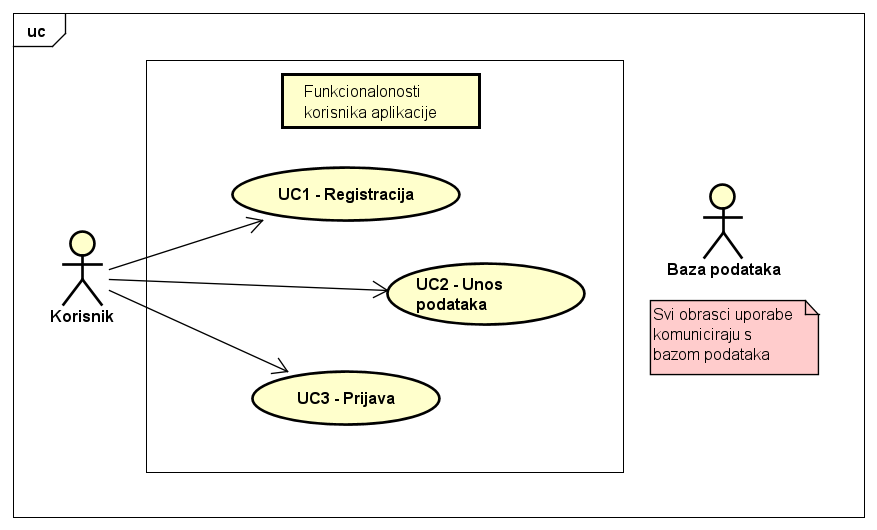
\includegraphics[scale=0.68]{dijagrami/UML_kor.PNG}
						\centering
						\caption{Dijagram obrasca uporabe, funkcionalnost korisnika}
						\label{fig:UML_kor}
					\end{figure}
				\eject
					
					\begin{figure}[h]
						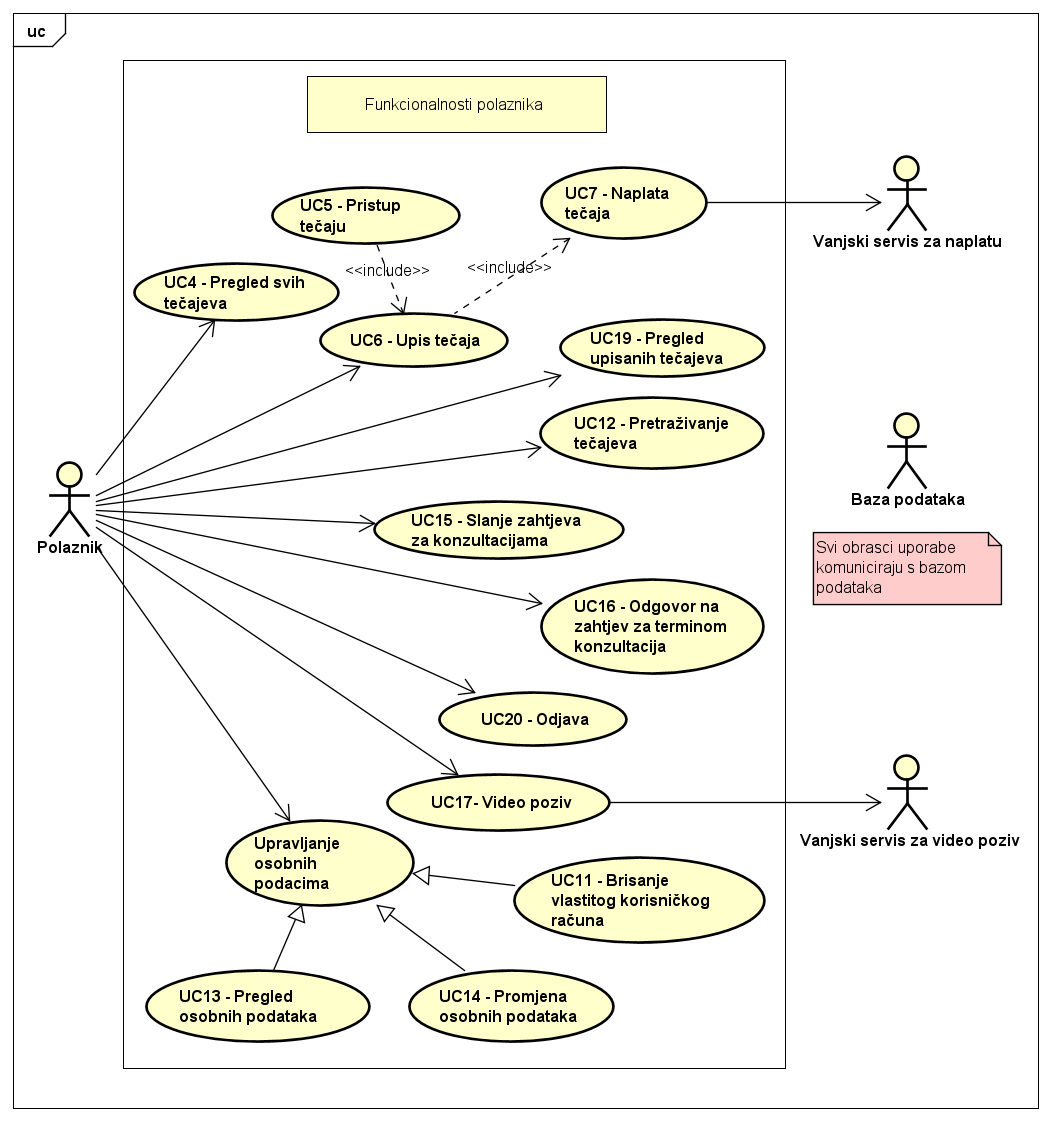
\includegraphics[scale=0.6]{dijagrami/UML_pol.PNG}
						\centering
						\caption{Dijagram obrasca uporabe, funkcionalnost polaznika tečaja}
						\label{fig:UML_pol}
					\end{figure}
				\eject
				
					\begin{figure}[h]
						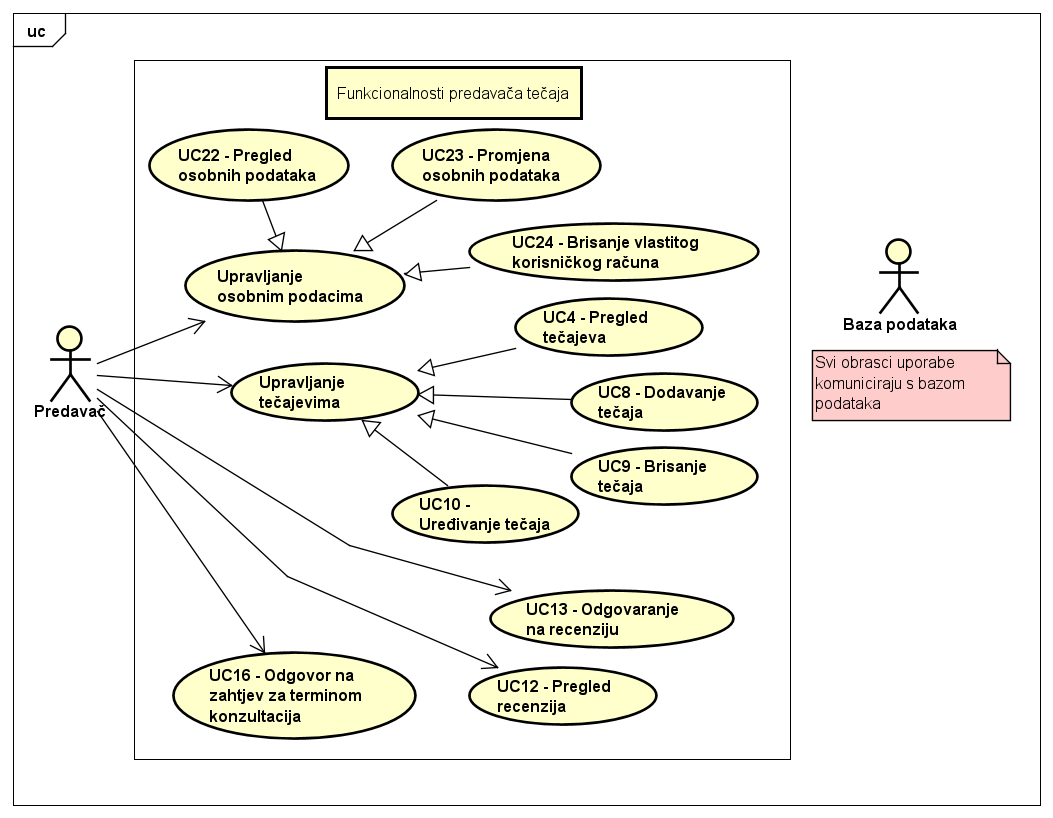
\includegraphics[scale=0.6]{dijagrami/UML_pred.PNG}
						\centering
						\caption{Dijagram obrasca uporabe, funkcionalnost predavača}
						\label{fig:UML_pred}
					\end{figure}
				\eject	
					\begin{figure}[h]
						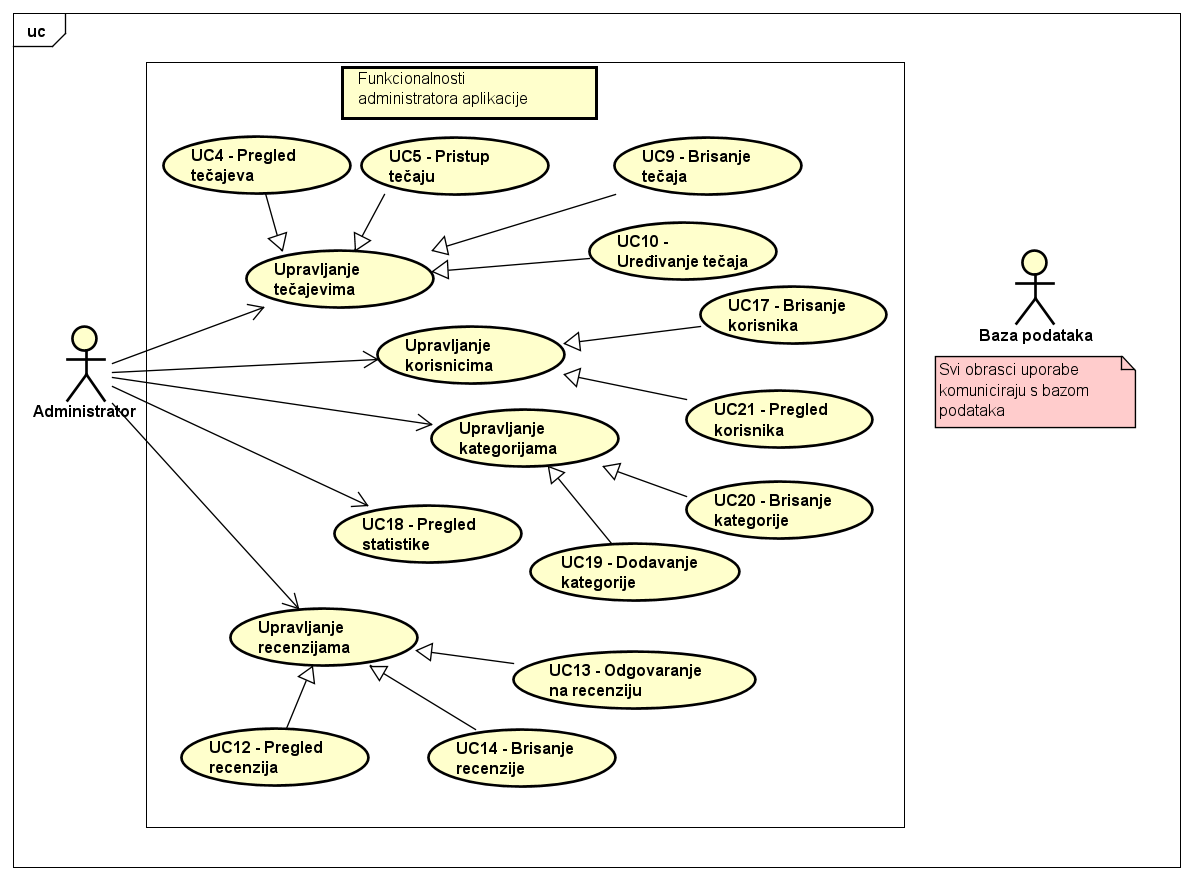
\includegraphics[scale=0.5]{dijagrami/UML_ad.PNG}
						\centering
						\caption{Dijagram obrasca uporabe, funkcionalnost administratora aplikacije}
						\label{fig:UML_ad}
					\end{figure}
				\eject		
				
			\subsection{Sekvencijski dijagrami}
				
				\subsubsection{Obrasci uporabe UC1 i UC2 - Registracija i Unos podataka}
				
					Korisnik unosi svoju e-mail adresu i željeno korisničko ime. Poslužitelj s bazom podataka provjerava jesu li unesena e-mail adresa i korisničko ime dostupni (nisu zauzeti od strane drugog korisnika). Poslužitelj također provjerava jesu li podaci u dozvoljenom formatu te je li navedena e-mail adresa ispravna. Ako podaci nisu ispravni, sustav korisniku šalje obavijest o neuspjelom upisu i vraća ga na ponovni unos podataka. Ako su podaci ispravni, korisnika se usmjerava na stranicu za unos dodatnih podataka. \newline
					Zatim korisnik unosi dodatne podatke. Ako su potrebni podaci ispravno uneseni, stvara se novi korisnički račun i korisnik dobiva obavijest o uspješnoj registraciji. Ako nije unesen jedan ili više potrebnih podataka, sustav obavještava korisnika. Ukoliko korisnik odluči odustati, registracija se briše.
				\eject
				
					\begin{figure}[h]
						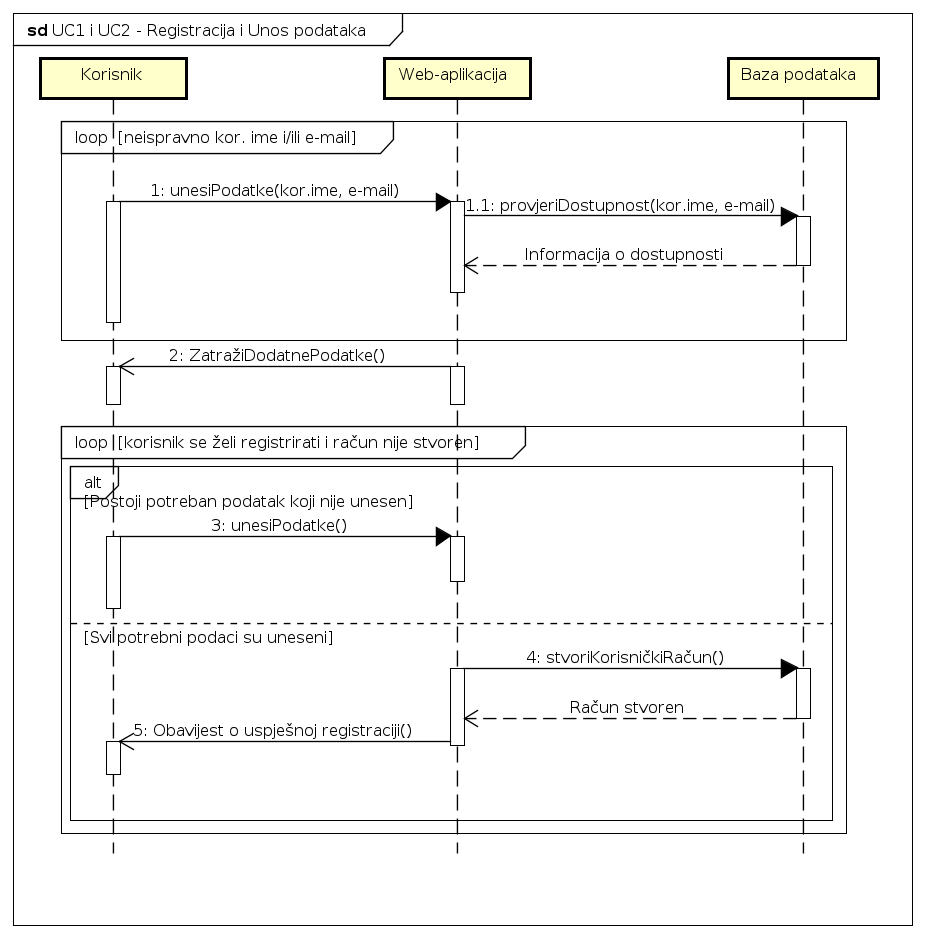
\includegraphics[scale=0.63]{dijagrami/UML_sd_UC1UC2.PNG}
						\centering
						\caption{Sekvencijski dijagram za UC1 i UC2}
						\label{fig:UML_sd_UC1UC2}
					\end{figure}
				
				\eject
				\subsubsection{Obrasci uporabe UC6 i UC7 - Upis tečaja i Naplata tečaja}
				
					Polaznik odabire tečaj koji želi upisati. Nakon odabira tečaja, sustav usmjerava polaznika na stranicu za naplatu. \newline
					Polaznik potvrđuje odabrani tečaj i iznos naplate, a zatim izvršava plaćanje tečaja. Ako na kartici ima dovoljno sredstava, tečaj se plaća i korisnik dobiva pristup tečaju. Ukoliko na kartici nema dovoljno sredstava, sustav obavještava korisnika o nemogućnosti pohađanja tečaja zbog financija.
				
					\begin{figure}[h]
						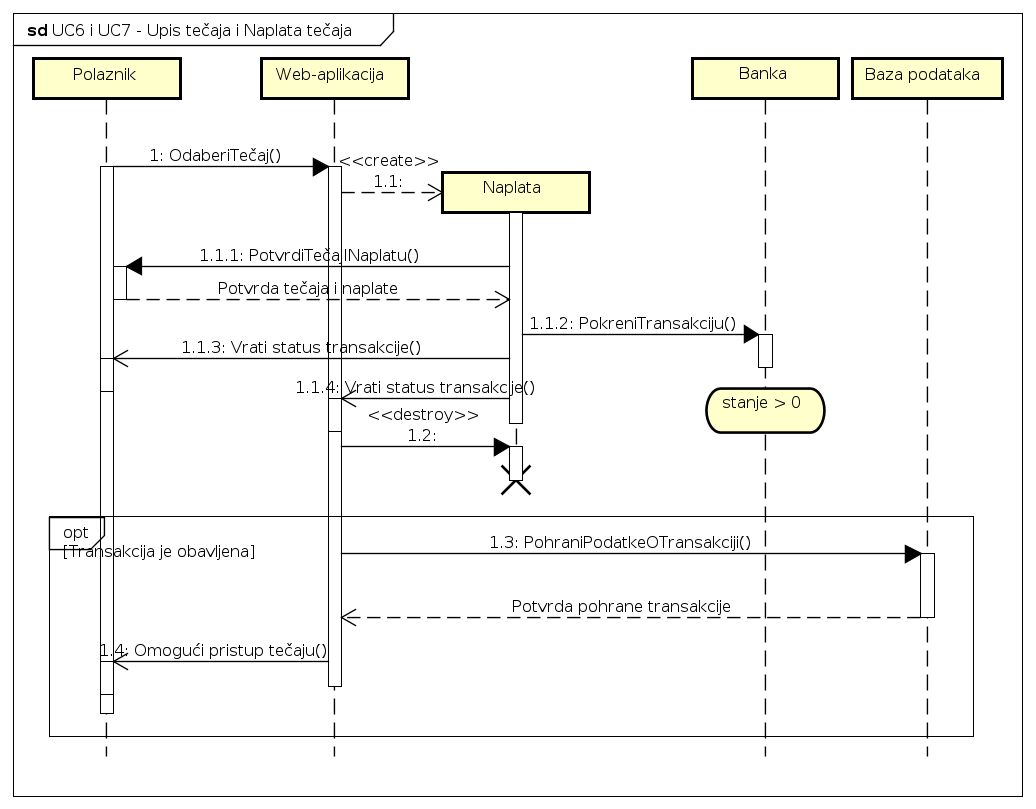
\includegraphics[scale=0.56]{dijagrami/UML_sd_UC6UC7.PNG}
						\centering
						\caption{Sekvencijski dijagram za UC6 i UC7}
						\label{fig:UML_sd_UC6UC7}
					\end{figure}
				
				\eject
				\subsubsection{Obrasci uporabe UC15 i UC16 - Slanje zahtjeva za konzultacijama i Odgovor na zahtjev za terminom konzultacija}
				
					Polaznik šalje zahtjev za terminom konzultacija. Podaci o zahtjevu se pohranjuju u bazu podataka. \newline
					Nakon što je zahtjev pohranjen u bazu podataka, 	poslužitelj predavaču šalje obavijest o dospjelom zahtjevu. Predavač šalje poslužitelju zahtjev za prikaz liste zahtjeva za terminima konzultacija. Poslužitelj dohvaća listu zahtjeva iz baze podataka i prikazuje ih predavaču. Predavač može prihvatiti ili odbiti predloženi termin konzultacija. Ako predavač prihvati termin, poslužitelj izmjenjuje zahtjev u bazi podataka koja vraća potvrdu o odobrenom zahtjevu. Poslužitelj tada šalje obavijest polazniku da je zahtjev odobren. Ako predavač odbije termin, poslužitelj briše poslani zahtjev iz baze podataka i obavještava polaznika da je zahtjev odbijen. Polaznik zatim ponovno šalje zahtjev za terminom konzultacija, sve dok mu se zahtjev ne odobri.
				\eject
				
					\begin{figure}[h]
						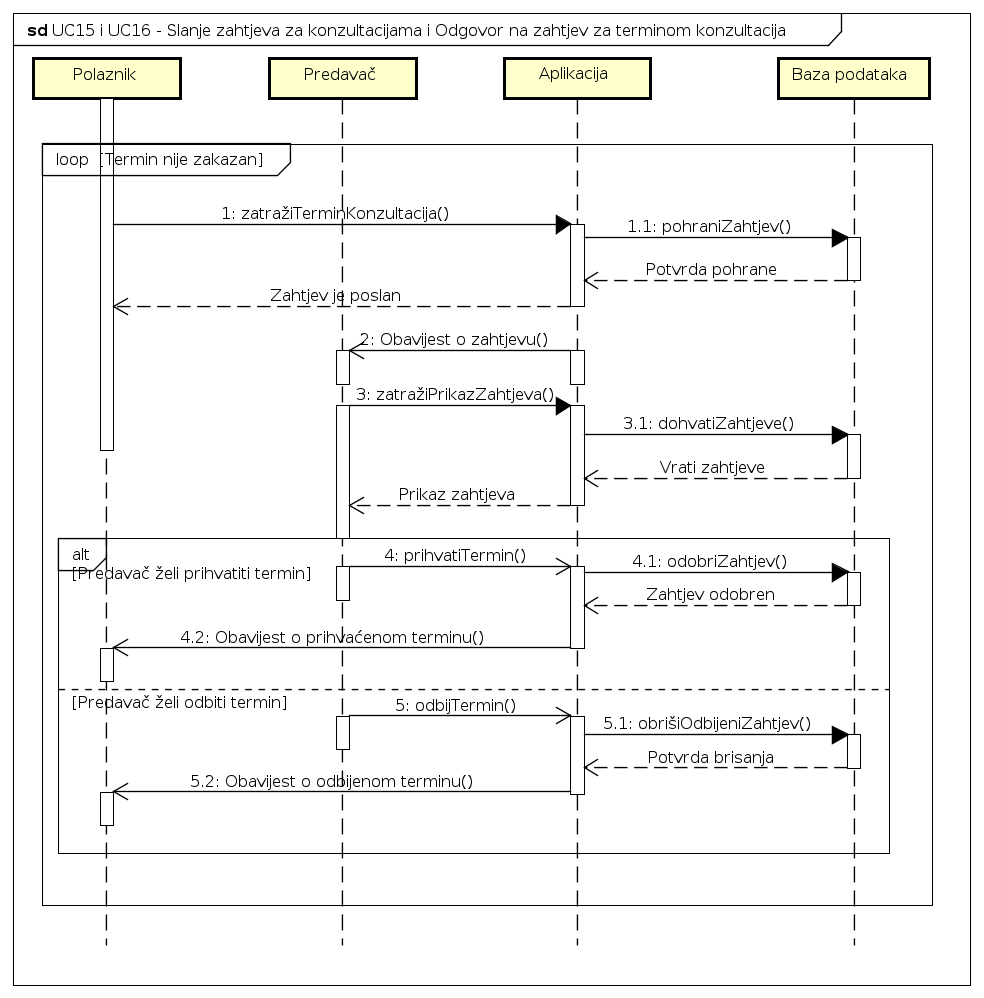
\includegraphics[scale=0.59]{dijagrami/UML_sd_UC15UC16.PNG}
						\centering
						\caption{Sekvencijski dijagram za UC15 i UC16}
						\label{fig:UML_sd_UC15UC16}
					\end{figure}
				\eject
				
		\section{Ostali zahtjevi}
		
			\begin{packed_item}
				\item Sustav treba podržavati rad više korisnika u isto vrijeme
				\item Sustav treba biti jednostavan za korištenje, korisnici se moraju znati koristiti sučeljem bez opširnih uputa
				\item Neispravno korištenje sučelja ne smije narušiti funkcionalnost i rad sustava
				\item Sustav kao valutu koristi HRK
				\item Nadogradnja sustava ne smije narušavati postojeće funkcionalnosti sustava
				\item Korisničko sučelje i sustav moraju podržavati hrvatsku abecedu (dijakritičke znakove) pri unosu i prikazu tekstualnog sadržaja
				\item Veza s bazom podataka mora biti kvalitetno zaštićena, brza i otporna na vanjske greške
				\item Aplikacija mora imati responzivno korisničko sučelje
				\item Svi osobni podaci u aplikaciji moraju se čuvati u skladu s GDPR regulativom
			\end{packed_item}
			 
			 
			 
	
	\chapter{Arhitektura i dizajn sustava}
		
		Arhitektura se može podijeliti na dva podsustava:
	\begin{itemize}
		\item Mobilna aplikacija
		\item Baza podataka
	\end{itemize}
	
	\begin{figure}[h]
		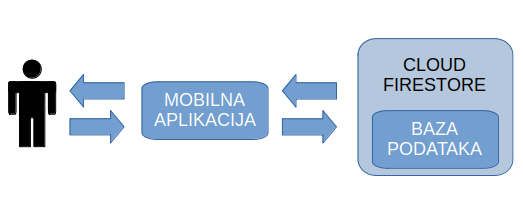
\includegraphics[scale=0.55]{slike/Arhitektura_sustava.PNG}
		\centering
		\caption{Arhitektura sustava}
		\label{fig:Arhitektura_sustava}
	\end{figure}
	
		\textit{\underbar{Mobilna aplikacija}} je program koji se izvodi na mobilnom uređaju. Mobilne aplikacije se uglavnom preuzimaju s distribucijskih platformi, nakon čega se provodi njihova instalacija. Korisnik koristi mobilnu aplikaciju za obrađivanje željenih zahtjeva, pri čemu aplikacija po potrebi pristupa bazi podataka.
		
		\textit{\underbar{Baza podatka}} je organizirani skup strukturiranih podataka. Za pohranu i pristup podacima koristi se računalni sustav.
		
		Za izradu naše mobilne aplikacije odabrali smo \href{https://flutter.dev/}{\textbf{Flutter}}, softver za razvoj korisničkog sučelja otvorenog koda koji je stvorio Google. Razlog zbog kojeg smo odabrali Flutter je jednostavnost izrade aplikacija i mogućnost višeplatformskog razvoja korištenjem jednog koda. Još jedna velika prednost je ta što se njime može realizirati i frontend i backend. Flutter koristi programski jezik Dart. Odabrano razvojno okruženje je Visual Studio Code.
		
		Baza podataka koju ćemo koristiti je \href{https://firebase.google.com/docs/firestore}{\textbf{Cloud Firestore}}. Cloud Firestore je NoSQL, dokumentno orijentirana baza podataka. Dokumenti su organizirani u kolekcije, a svaki dokument ima svoje ime (koje služi kao identifikator) i skup atributa kojima su pridružene vrijednosti. Glavne prednosti ovakve organizacije su efikasni upiti i velika brzina rada. Cloud Firestore omogućuje iOS, Android i web aplikacijama izravan pristup putem njihovih vlastitih programskih alata.
		
		Arhitektura sustava temeljiti će se na MVVM (Model-View-ViewModel) konceptu. Karakteristika MVVM koncepta je podjela na komponente čiji nezavisni razvoj osigurava fleksibilnost, smanjuje međuovisnost, povećava ponovnu uporabivost i pojednostavljuje ispitivanje. \newline
		MVVM koncept se sastoji od:
	\begin{itemize}
		\item \textbf{\underline{Model}} - Pohranjuje podatke i informacije potrebne za rad aplikacije. Odvojen je od logičkog dijela koji određuje prikaz podataka i usluga koje njima manipuliraju.
		\item \textbf{\underline{View}} - Predstavlja sučelje koje korisnik vidi u interakciji s aplikacijom. Identificira i reagira na korisničke akcije.
		\item \textbf{\underline{ViewModel}} - Središnja komponenta sustava. Služi kao sučelje između Modela i Viewa. Šalje i prima podatke od Modela te osigurava podatke potrebne Viewu. Također, promatra promjene koje se događaju u Viewu. Raspolaže metodama koje održavaju stanja Viewa i upravlja podacima u Modelu.
	\end{itemize}
		
	\eject

				
		\section{Baza podataka}
			
			\text Za potrebe našeg sustava koristit ćemo NoSQL bazu podataka orijentiranu na dokumente, odnosno kolekcije dokumenata. Gradivna jedinka baze je dokument koji je definiran svojim imenom i skupom atributa. Zadaća baze podataka jest jednostavna i brza pohrana, izmjena i dohvat podataka za daljnju obranu. Baza podataka ove aplikacije sastoji se od tri entiteta, a to su:
			
			\begin{itemize}
				\item User
				\item Categories
				\item Meetings
			\end{itemize}
		
			\subsection{Opis tablica}
			

				\textbf{User} \text    Ovaj entitet sadržava sve važne informacije o korisniku aplikacije. Sadrži atribute: about, cardExp, creditCard, firstName, iban, image, lastName, lecturer, mail, secCode, username. Za svakog novog registriranog korisnika kreira se dokument pod šifrom u bazi podataka.
				
				\begin{longtabu} to \textwidth {|X[6, l]|X[6, l]|X[20, l]|}
					
					\hline \multicolumn{3}{|c|}{\textbf{User}}	 \\[3pt] \hline
					\endfirsthead
					
					\hline \multicolumn{3}{|c|}{\textbf{User}}	 \\[3pt] \hline
					\endhead
					
					\hline 
					\endlastfoot
					
					Mail & string & mail korisnika \\ \hline
					Username & string & korisničko ime \\ \hline
					Lecturer & boolean & oznaka je li korisnik registriran kao predavač \\ \hline
					FirstName & string & ime korisnika \\ \hline
					LastName & string & prezime korisnika \\ \hline
					CardExp & string & datum isteka kartice za naplatu \\ \hline
					CreditCard & string & broj kartice za naplatu \\ \hline
					SecCode & string & kod za verifikaciju kartice \\ \hline
					iban & string & IBAN računa za isplatu honorara \\ \hline
					About & string & kratka biografija o korisniku ukoliko je predavač \\ \hline
					Image & string & poveznica na fotografiju korisnika ukoliko je predavač \\ \hline
					Courses & array & sadrži sve tečajeve koje je korisnik upisao (za polaznika) ili koje je kreirao (za predavača) \\ \hline					
				\end{longtabu}
			
			\textbf{Categories} \text    Ovaj entitet sadržava sve važne informacije o tečajevima koji su dostupni na aplikaciji. Sadrži atribut name te kolekciju za svaku razinu tečaja (beginner, intermediate, advanced) koja će sadržavati dodatne informacije o pojedinom tečaju. Za svaku kategoriju tečaja kreiran je dokument u bazi podataka, a za svaki tečaj kreira se dokument unutar kolekcije za odrabranu razinu i kategoriju tečaja. 
			
			\begin{longtabu} to \textwidth {|X[6, l]|X[6, l]|X[20, l]|}
				
				\hline \multicolumn{3}{|c|}{\textbf{Categories}}	 \\[3pt] \hline
				\endfirsthead
				
				\hline \multicolumn{3}{|c|}{\textbf{Categories}}	 \\[3pt] \hline
				\endhead
				
				\hline 
				\endlastfoot
				
				Name & string & naziv kategorije tečaja \\ \hline
				Difficulty & kolekcija & sadrži tri moguće razine tečajeva: početnička, srednja i napredna \\ \hline					
				
			\end{longtabu}
		
			\textbf{Difficulty} \text    Ova kolekcija unutar entiteta Courses sadrži kolekcije tečajeva (pod određenom kategorijom) raspoređene po razinama. 
			
			\begin{longtabu} to \textwidth {|X[6, l]|X[6, l]|X[20, l]|}
				
				\hline \multicolumn{3}{|c|}{\textbf{Difficulty}}	 \\[3pt] \hline
				\endfirsthead
				
				\hline \multicolumn{3}{|c|}{\textbf{Difficulty}}	 \\[3pt] \hline
				\endhead
				
				\hline 
				\endlastfoot
				
				Beginner & kolekcija & početnička razina tečaja \\ \hline
				Advanced & kolekcija & napredna razina tečaja \\ \hline
				Intermediate & kolekcija & srednja razina tečaja \\ \hline					
				
			\end{longtabu}
		
		
				\textbf{Beginner/Advanced/Intermediate} \text    Ove kolekcije sadrže informacije o tečaju koje su nužne za njegovo kreiranje. 
			
			\begin{longtabu} to \textwidth {|X[8, l]|X[6, l]|X[20, l]|}
				
				\hline \multicolumn{3}{|c|}{\textbf{Beginner/Advanced/Intermediate}}	 \\[3pt] \hline
				\endfirsthead
				
				\hline \multicolumn{3}{|c|}{\textbf{Beginner/Advanced/Intermediate}}	 \\[3pt] \hline
				\endhead
				
				\hline 
				\endlastfoot
				
				CourseInfo & string & kratki opis tečaja (do 1000 riječi) \\ \hline
				CourseMail & string & e-mail adresa vlasnika tečaja \\ \hline
				CourseMaterials & array & materijali za učenje (PDF format do 50 MB ukupno) \\ \hline
				CourseName & string & naziv tečaja \\ \hline
				CoursePrice & number & cijena tečaja \\ \hline
				Keywords & array & ključne riječi po kojima je moguće pronaći tečaj \\ \hline
								
				
			\end{longtabu}
		\eject
		
			\textbf{Meetings} \text    Ovaj entitet sadržava sve važne informacije o zatraženim konzultacijama. 
			
			\begin{longtabu} to \textwidth {|X[9, l]|X[6, l]|X[20, l]|}
				
				\hline \multicolumn{3}{|c|}{\textbf{Meetings}}	 \\[3pt] \hline
				\endfirsthead
				
				\hline \multicolumn{3}{|c|}{\textbf{Meetings}}	 \\[3pt] \hline
				\endhead
				
				\hline 
				\endlastfoot
				
				CourseID & string & ID dokumenta u bazi podataka za odabrani tečaj  \\ \hline
				LecturerConfirm & boolean & oznaka da je predavač potvrdio termin konzultacija \\ \hline
				LecturerMail & string & e-mail predavača \\ \hline
				ReqDate & string & traženi datum konzultacija \\ \hline
				StudentConfirm & boolean & oznaka da je polaznik potvrdio termin konzultacija \\ \hline
				StudentMail & string & e-mail polaznika koji je zatražio konzultacije \\ \hline				
				
			\end{longtabu}
			\pagebreak
			
			\subsection{Dijagram baze podataka}
				\begin{figure}[H]
					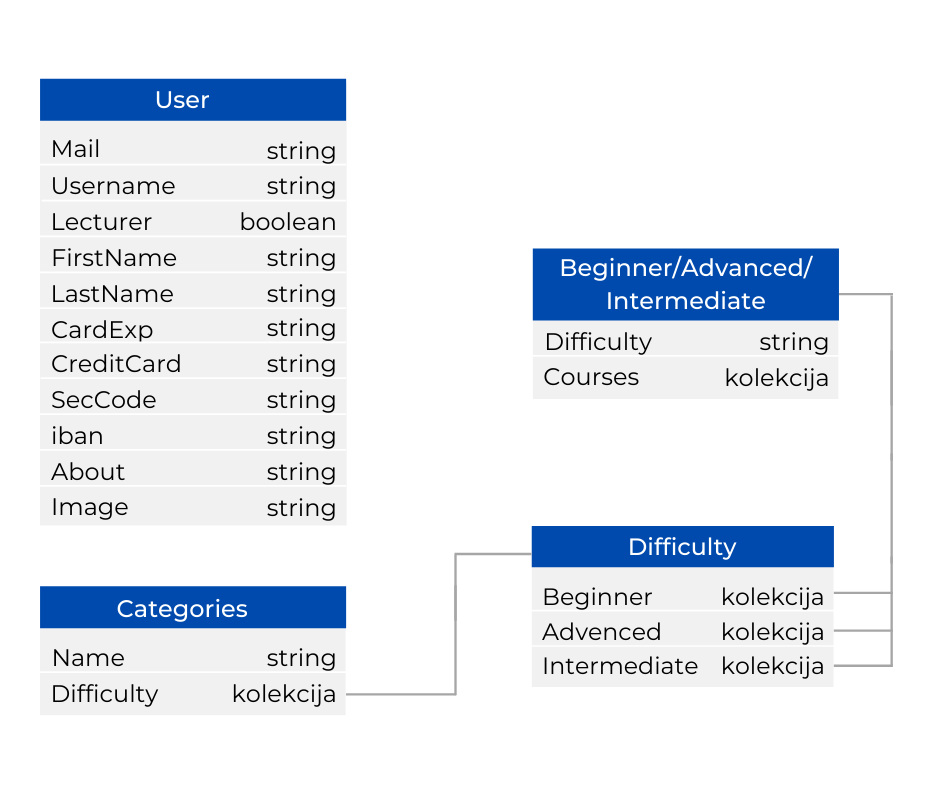
\includegraphics[scale=0.6]{dijagrami/ER_baza_podataka.PNG} 
					\centering
					\caption{E-R dijagram baze podataka}
					\label{fig:ER}
				\end{figure} 
			
			\eject
			
			
		\section{Dijagram razreda}
		
			Na slici \ref{fig:ViewModel} su prikazani razredi koji pripadaju \textit{backend} dijelu MVVM arhitekture. Funkcije implementirane u razredima ConsultationDB, CoursesDB i UserInfoDB manipuliraju podacima u bazi podataka koja predstavlja Model komponentu arhitekture. Sve funkcije koje manipuliraju podacima u bazi podataka (i općenito rade s Firebase metodama) su tipa Future, što znači da su te funkcije asinkrone zbog vremenski zahtjevnih procedura.
			
			
			\begin{figure}[h]
				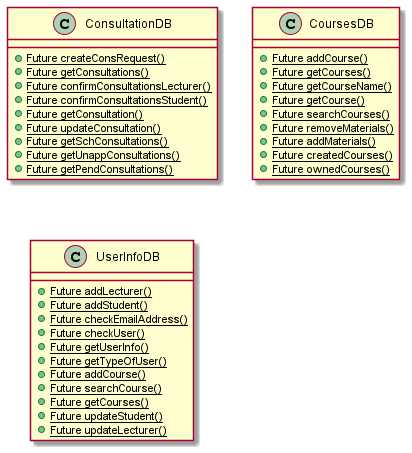
\includegraphics[scale=0.8]{dijagrami/ViewModel.PNG}
				\centering
				\caption{Dijagram razreda - dio ViewModel}
				\label{fig:ViewModel}
			\end{figure}
			
			Na slici \ref{fig:View3} su prikazani razredi koji pripadaju \textit{frontend} dijelu MVVM arhitekture. View razredi služe za prikaz podataka korisniku. Svi View razredi su implementirani kao State, što znači da se njihov prikaz osvježava sa svakom promjenom stanja razreda.
			
			Zbog lakšeg prikaza, dijagram razreda View komponente je podijeljen na tri dijela, koji su prikazani jedan ispod drugog.
			
			\eject
			\begin{figure}[h]
				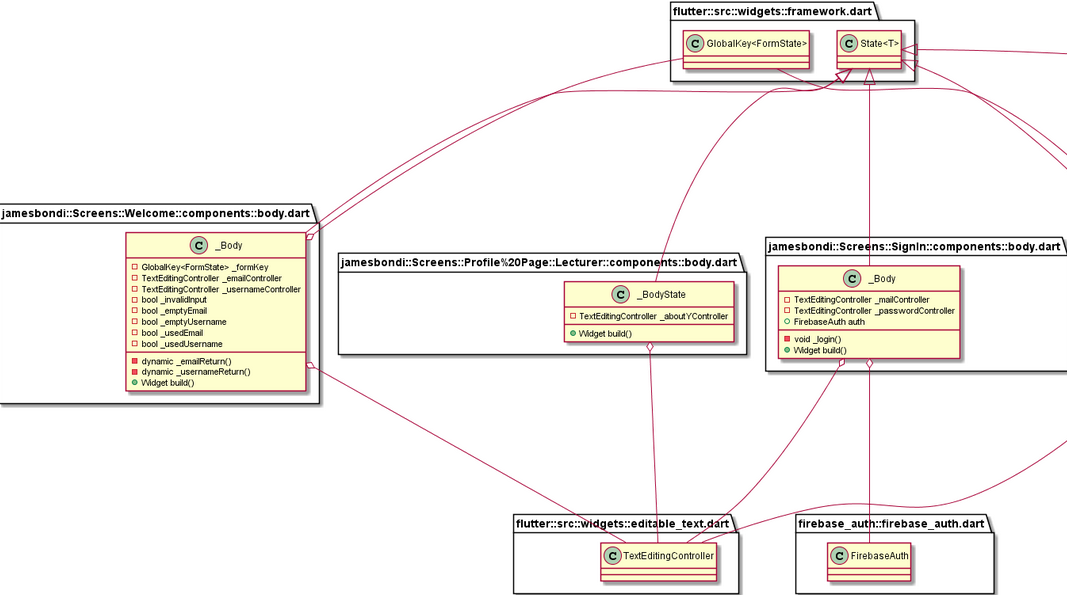
\includegraphics[scale=0.41]{dijagrami/View1.PNG}
				\centering
			\end{figure}
			
			\begin{figure}[h]
				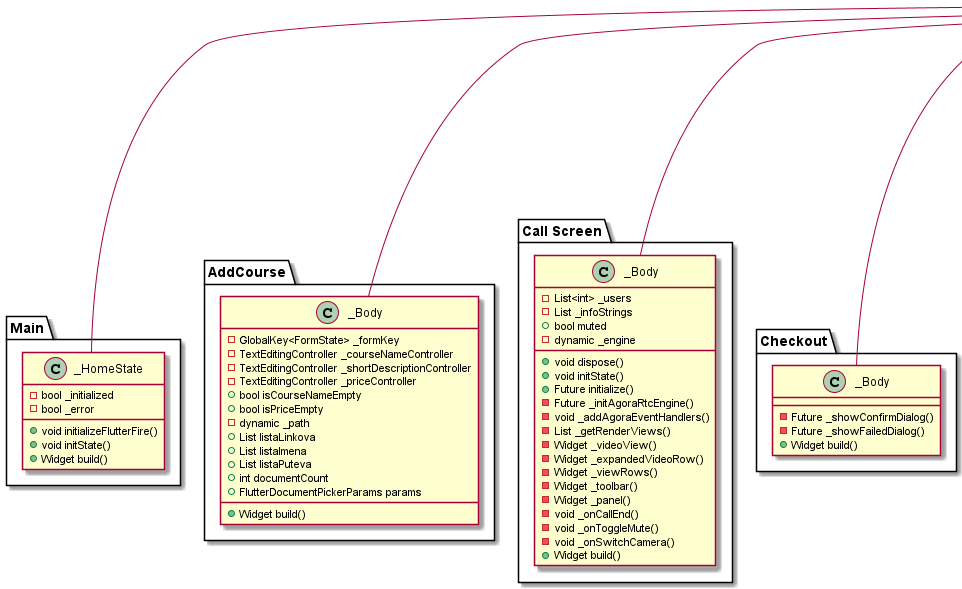
\includegraphics[scale=0.44]{dijagrami/View2.PNG}
				\centering
			\end{figure}
			
			\begin{figure}[hbt!]
				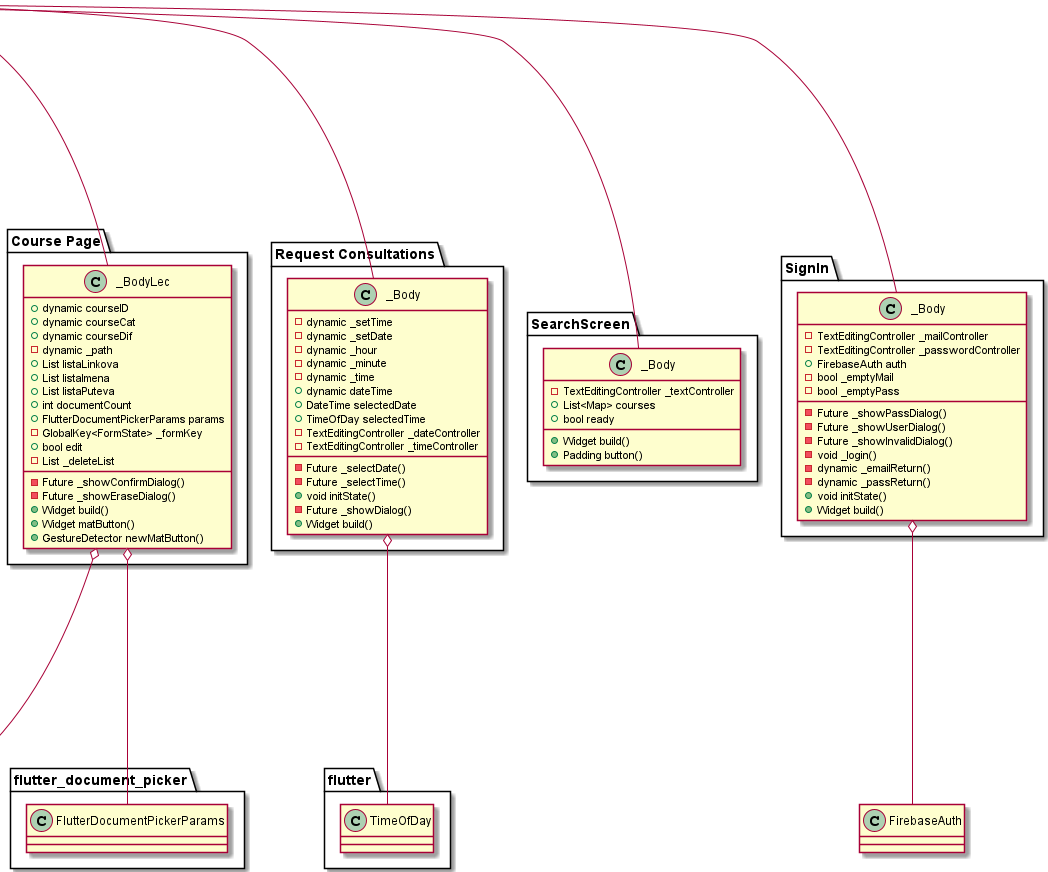
\includegraphics[scale=0.4]{dijagrami/View3.PNG}
				\centering
				\caption{Dijagram razreda - dio View}
				\label{fig:View3}
			\end{figure}
			
			\eject
			
		\section{Dijagram stanja}
			
			
			Dijagram stanja prikazuje stanja objekta te prijelaze iz jednog stanja u drugo temeljene na događajima. Na slici \ref{fig:Dijagram_stanja} prikazan je dijagram stanja za korisnika koji je registriran kao polaznik. Nakon prijave, polazniku se prikazuje početna stranica na kojoj su navedene kategorije tečajeva. Dodirom na željenu kategoriju polazniku se prikazuje izbornik u kojem odabire težinu tečaja. Aplikacija će zatim prikazati tečajeve koji zadovoljavaju zahtjeve polaznika. Pretraživanje tečajeva moguće je provesti i unosom ključnih riječi u pretraživač kojem se pristupa dodirom na "Search". Dodirom na tečaj prikazuju se njegove informacije. Ako polaznik odabere neupisani tečaj, ima opciju pregleda profila predavača i opciju upisa tečaja koji uključuje naplatu korištenjem vanjskog servisa. Odabirom već upisanog tečaja polazniku se također nudi opcija pregleda profila predavača, kao i opcija preuzimanja materijala. Dodirom na "Ask for consultations" otvara se izbornik koji omogućuje zatraživanje novog termina konzultacija.
			
			Upravljanje konzultacijama polazniku je dostupno dodirom na "Consultations". Na vrhu stranice nalazi se lista termina konzultacija dogovorenih s predavačem. Listu je moguće osvježiti dodirom na "Refresh". Videopoziv se započinje dodirom na "consultations" pokraj pripadnog dogovorenog termina. Na stranici su također prikazani termini konzultacija ponuđeni od strane predavača. Ponuđeni termin moguće je prihvatiti ili odbiti. Ako polaznik prihvati termin, on se pojavljuje u listi dogovorenih termina. U slučaju odbijanja termina, polazniku se otvara izbornik u kojem je moguće predložiti novi termin konzultacija.
			
			Dodirom na "Profile" polazniku se otvara prikaz osobnih podataka. Polaznik ima opciju izmijeniti osobne podatke dodirom na "Edit your profile", kao i opciju prikaza upisanih tečajeva dodirom na "Show owned courses". Odjava se provodi dodirom na "Sign out".
			
			\eject
			
			\begin{figure}[h]
				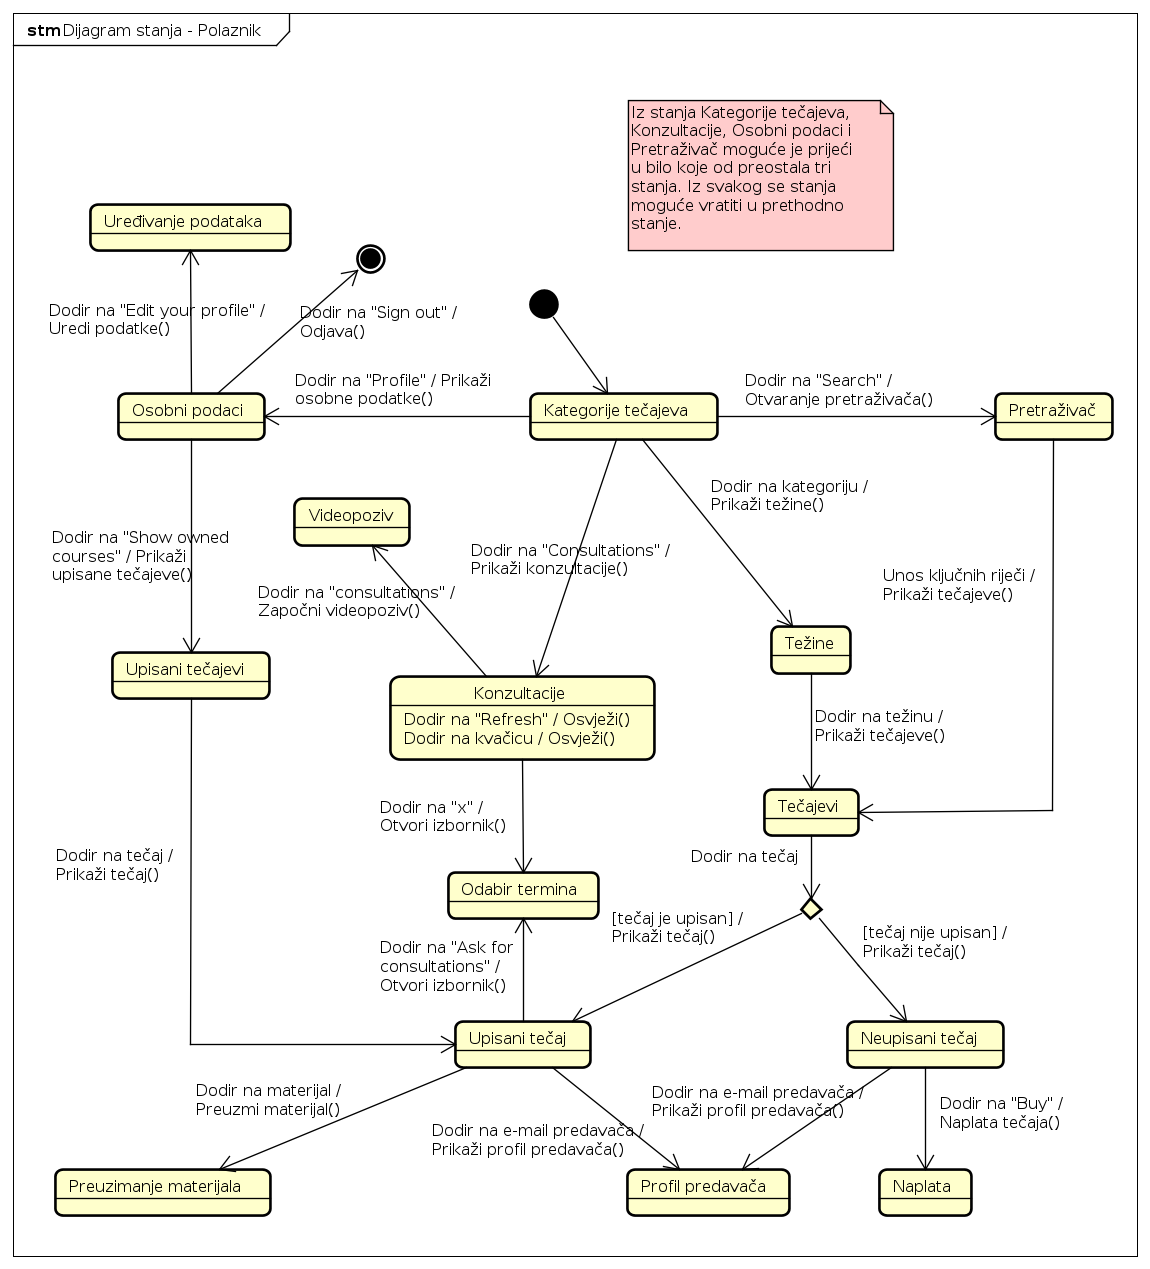
\includegraphics[scale=0.5]{dijagrami/Dijagram_stanja.PNG}
				\centering
				\caption{Dijagram stanja - Polaznik}
				\label{fig:Dijagram_stanja}
			\end{figure}
		
		
			\eject 
		
		\section{Dijagram aktivnosti}
			
			\textbf{\textit{dio 2. revizije}}\\
			
			 \textit{Potrebno je priložiti dijagram aktivnosti s pripadajućim opisom. Dijagram aktivnosti treba prikazivati značajan dio sustava.}
			
			\eject
		\section{Dijagram komponenti}
		
			\textbf{\textit{dio 2. revizije}}\\
		
			 \textit{Potrebno je priložiti dijagram komponenti s pripadajućim opisom. Dijagram komponenti treba prikazivati strukturu cijele aplikacije.}
	\chapter{Implementacija i korisničko sučelje}
		
		
		\section{Korištene tehnologije i alati}
		
			\textbf{\textit{dio 2. revizije}}
			
			 \textit{Detaljno navesti sve tehnologije i alate koji su primijenjeni pri izradi dokumentacije i aplikacije. Ukratko ih opisati, te navesti njihovo značenje i mjesto primjene. Za svaki navedeni alat i tehnologiju je potrebno \textbf{navesti internet poveznicu} gdje se mogu preuzeti ili više saznati o njima}.
			
			
			\eject 
		
	
		\section{Ispitivanje programskog rješenja}
			
			\textbf{\textit{dio 2. revizije}}\\
			
			 \textit{U ovom poglavlju je potrebno opisati provedbu ispitivanja implementiranih funkcionalnosti na razini komponenti i na razini cijelog sustava s prikazom odabranih ispitnih slučajeva. Studenti trebaju ispitati temeljnu funkcionalnost i rubne uvjete.}
	
			
			\subsection{Ispitivanje komponenti}
			\textit{Potrebno je provesti ispitivanje jedinica (engl. unit testing) nad razredima koji implementiraju temeljne funkcionalnosti. Razraditi \textbf{minimalno 6 ispitnih slučajeva} u kojima će se ispitati redovni slučajevi, rubni uvjeti te izazivanje pogreške (engl. exception throwing). Poželjno je stvoriti i ispitni slučaj koji koristi funkcionalnosti koje nisu implementirane. Potrebno je priložiti izvorni kôd svih ispitnih slučajeva te prikaz rezultata izvođenja ispita u razvojnom okruženju (prolaz/pad ispita). }
			
			
			
			\subsection{Ispitivanje sustava}
			
			 \textit{Potrebno je provesti i opisati ispitivanje sustava koristeći radni okvir Selenium\footnote{\url{https://www.seleniumhq.org/}}. Razraditi \textbf{minimalno 4 ispitna slučaja} u kojima će se ispitati redovni slučajevi, rubni uvjeti te poziv funkcionalnosti koja nije implementirana/izaziva pogrešku kako bi se vidjelo na koji način sustav reagira kada nešto nije u potpunosti ostvareno. Ispitni slučaj se treba sastojati od ulaza (npr. korisničko ime i lozinka), očekivanog izlaza ili rezultata, koraka ispitivanja i dobivenog izlaza ili rezultata.\\ }
			 
			 \textit{Izradu ispitnih slučajeva pomoću radnog okvira Selenium moguće je provesti pomoću jednog od sljedeća dva alata:}
			 \begin{itemize}
			 	\item \textit{dodatak za preglednik \textbf{Selenium IDE} - snimanje korisnikovih akcija radi automatskog ponavljanja ispita	}
			 	\item \textit{\textbf{Selenium WebDriver} - podrška za pisanje ispita u jezicima Java, C\#, PHP koristeći posebno programsko sučelje.}
			 \end{itemize}
		 	\textit{Detalji o korištenju alata Selenium bit će prikazani na posebnom predavanju tijekom semestra.}
			
			\eject 
		
		
		\section{Dijagram razmještaja}
			
			\textbf{\textit{dio 2. revizije}}
			
			 \textit{Potrebno je umetnuti \textbf{specifikacijski} dijagram razmještaja i opisati ga. Moguće je umjesto specifikacijskog dijagrama razmještaja umetnuti dijagram razmještaja instanci, pod uvjetom da taj dijagram bolje opisuje neki važniji dio sustava.}
			
			\eject 
		
		\section{Upute za puštanje u pogon}
		
			\textbf{\textit{dio 2. revizije}}\\
		
			 \textit{U ovom poglavlju potrebno je dati upute za puštanje u pogon (engl. deployment) ostvarene aplikacije. Na primjer, za web aplikacije, opisati postupak kojim se od izvornog kôda dolazi do potpuno postavljene baze podataka i poslužitelja koji odgovara na upite korisnika. Za mobilnu aplikaciju, postupak kojim se aplikacija izgradi, te postavi na neku od trgovina. Za stolnu (engl. desktop) aplikaciju, postupak kojim se aplikacija instalira na računalo. Ukoliko mobilne i stolne aplikacije komuniciraju s poslužiteljem i/ili bazom podataka, opisati i postupak njihovog postavljanja. Pri izradi uputa preporučuje se \textbf{naglasiti korake instalacije uporabom natuknica} te koristiti što je više moguće \textbf{slike ekrana} (engl. screenshots) kako bi upute bile jasne i jednostavne za slijediti.}
			
			
			 \textit{Dovršenu aplikaciju potrebno je pokrenuti na javno dostupnom poslužitelju. Studentima se preporuča korištenje neke od sljedećih besplatnih usluga: \href{https://aws.amazon.com/}{Amazon AWS}, \href{https://azure.microsoft.com/en-us/}{Microsoft Azure} ili \href{https://www.heroku.com/}{Heroku}. Mobilne aplikacije trebaju biti objavljene na F-Droid, Google Play ili Amazon App trgovini.}
			
			
			\eject 
	\chapter{Zaključak i budući rad}
		
		\text Zadatak naše grupe bio je razvoj mobilne aplikacije putem koje se mogu održavati online tečajevi koji će obuhvaćati unaprijed pripremljene materijale (videosnimke, skripte i prezentacije) uz mogućnost održavanja konzultacija uživo putem video poziva unutar aplikacije. Nakon 17 tjedana rada u timu i razvoja, ostvarili smo zadani cilj. Provedba projekta tekla je kroz dvije faze.
		
		\text Prva faza projekta uključivala je okupljanje tima za razvoj aplikacije, dodjelu projektnog zadatka, podjelu odgovornosti i dužnosti, rad na dokumentiranju zahtjeva te razvoj osnovnih funkcionalnosti aplikacije (kreiranje korisničkog računa, prijava u aplikaciju i slično). Paralelno smo izrađivali aplikaciju i dokumentaciju, što je rezultiralo manjim pritiskom na članove tima približavanjem zadanih rokova. Podjela posla uvelike je olakšala rad u grupi te smanjila potrebu za sastancima.		
		
		Druga faza projekta bila je nešto kraća od prve. Tijekom ove faze projekta, nastojali smo realizirati napredne funkcionalnosti aplikacije – kreiranje tečaja, dogovaranje konzultacija, uspostava video poziva unutar aplikacije te sam upis tečaja. Također, u ovoj fazi potrebno je bilo ispitati naše programsko rješenje i pustiti aplikaciju u pogon.
		
		Komunikacija među članovima tima odvijala se putem WhatsApp-a i Messengera za Facebook, kako bismo postigli informiranost svih članova tima o napretku projekta.  Moguće proširenje postojeće inačice aplikacije jest sustav obavijesti, koji bi podsjećao korisnike na dogovorene konzultacije, nove dostupne materijale i slično.
		
		Sudjelovanje na ovakvom projektu bilo je vrijedno iskustvo svim članovima, budući da je većini ovo bio prvi susret s radom u timu na istom projektu. Kroz nekoliko intenzivnih tjedana rada iskusili smo važnost dobre organizacije i komunikacije. Zadovoljni smo postignutim rješenjem, iako postoji veliki prostor za napredak aplikacije.
		
		
		\eject 
	\chapter*{Popis literature}
		\addcontentsline{toc}{chapter}{Popis literature}
	 	
 		\textbf{\textit{Kontinuirano osvježavanje}}
	
		\textit{Popisati sve reference i literaturu koja je pomogla pri ostvarivanju projekta.}
		
		
		\begin{enumerate}
			
			
			\item  Programsko inženjerstvo, FER ZEMRIS, \url{http://www.fer.hr/predmet/proinz}
			
			\item  I. Sommerville, "Software engineering", 8th ed, Addison Wesley, 2007.
			
			\item  T.C.Lethbridge, R.Langaniere, "Object-Oriented Software Engineering", 2nd ed. McGraw-Hill, 2005.
			
			\item  I. Marsic, Software engineering book``, Department of Electrical and Computer Engineering, Rutgers University, \url{http://www.ece.rutgers.edu/~marsic/books/SE}
			
			\item  The Unified Modeling Language, \url{https://www.uml-diagrams.org/}
			
			\item  Astah Community, \url{http://astah.net/editions/uml-new}
		\end{enumerate}
		
		 
	
	
	\begingroup
	\renewcommand*\listfigurename{Indeks slika i dijagrama}
	%\renewcommand*\listtablename{Indeks tablica}
	%\let\clearpage\relax
	\listoffigures
	%\vspace{10mm}
	%\listoftables
	\endgroup
	\addcontentsline{toc}{chapter}{Indeks slika i dijagrama}


	
	\eject 
		
	\chapter*{Dodatak: Prikaz aktivnosti grupe}
		\addcontentsline{toc}{chapter}{Dodatak: Prikaz aktivnosti grupe}
		
		\section*{Dnevnik sastajanja}
		
		
		\begin{packed_enum}
			\item  sastanak
			
			\item[] \begin{packed_item}
				\item Datum: 05. listopada 2020.
				\item Prisustvovali: D.Begić, G.Brkić, M.Dodik, M.Fabijanić, S.Gojević, A.Sabljić, V.Sokolić
				\item Teme sastanka:
				\begin{packed_item}
					\item  sastanak s asistenticom Nikolinom Frid
					\item  analiza zadatka
					\item raščišćavanje dilema funkcionalnosti
				\end{packed_item}
			\end{packed_item}
			
			\item  sastanak
			\item[] \begin{packed_item}
				\item Datum: 10. listopada 2020.
				\item Prisustvovali: D. Begić, G. Brkić, M. Dodik, M. Fabijanić, S. Gojević, A. Sabljić, V. Sokolić
				\item Teme sastanka:
				\begin{packed_item}
					\item  odabir alata i tehnologija
					\item  podjela dužnosti i poslova
				\end{packed_item}
			\end{packed_item}
		
			\item  sastanak
			\item[] \begin{packed_item}
				\item Datum: 18. listopada 2020.
				\item Prisustvovali: D. Begić, G. Brkić, M. Dodik, M. Fabijanić, S. Gojević, A. Sabljić, V. Sokolić
				\item Teme sastanka:
				\begin{packed_item}
					\item  definiranje funkcionalnih zahtjeva
					\item  definiranje obrazaca uporabe
				\end{packed_item}
			\end{packed_item}
			
			\item  sastanak
			\item[] \begin{packed_item}
				\item Datum: 02. studeni 2020.
				\item Prisustvovali: D.Begić, G.Brkić, M.Dodik, M.Fabijanić, S.Gojević, A.Sabljić, V.Sokolić
				\item Teme sastanka:
				\begin{packed_item}
					\item  sastanak s asistenticom Nikolinom Frid
					\item  raščišćavanje dilema opisa obrazaca uporabe
					\item demonstracija postignute funkcionalnosti
				\end{packed_item}
			\end{packed_item}
		
			\item  sastanak
			\item[] \begin{packed_item}
				\item Datum: 09. studeni 2020.
				\item Prisustvovali: D.Begić, G.Brkić, M.Dodik, M.Fabijanić, S.Gojević, A.Sabljić, V.Sokolić
				\item Teme sastanka:
				\begin{packed_item}
					\item  sastanak s asistenticom Nikolinom Frid
					\item  evaluacija dosadašnjeg rada
					\item raščišćavanje dilema baze podataka
				\end{packed_item}
			\end{packed_item}
			%
			
		\end{packed_enum}
		
		\eject
		\section*{Tablica aktivnosti}
	
			
			\begin{longtabu} to \textwidth {|X[7, l]|X[1, c]|X[1, c]|X[1, c]|X[1, c]|X[1, c]|X[1, c]|X[1, c]|}
								
				\cline{2-8} \multicolumn{1}{c|}{\textbf{}} &     \multicolumn{1}{c|}{\rotatebox{90}{\textbf{Marin Fabijanić }}} & \multicolumn{1}{c|}{\rotatebox{90}{\textbf{Dominik Begić }}} &	\multicolumn{1}{c|}{\rotatebox{90}{\textbf{Goran Brkić }}} &	\multicolumn{1}{c|}{\rotatebox{90}{\textbf{Marko Dodik }}} &
				\multicolumn{1}{c|}{\rotatebox{90}{\textbf{Silvija Gojević }}} &
				\multicolumn{1}{c|}{\rotatebox{90}{\textbf{Antonio Sabljić }}} &	\multicolumn{1}{c|}{\rotatebox{90}{\textbf{Vlatko Sokolić }}} \\ \hline 
				\endfirsthead
				
			
				\cline{2-8} \multicolumn{1}{c|}{\textbf{}} &     \multicolumn{1}{c|}{\rotatebox{90}{\textbf{Marin Fabijanić}}} & \multicolumn{1}{c|}{\rotatebox{90}{\textbf{Dominik Begić }}} &	\multicolumn{1}{c|}{\rotatebox{90}{\textbf{Goran Brkić }}} &
				\multicolumn{1}{c|}{\rotatebox{90}{\textbf{Marko Dodik }}} &	\multicolumn{1}{c|}{\rotatebox{90}{\textbf{Silvija Gojević }}} &
				\multicolumn{1}{c|}{\rotatebox{90}{\textbf{Antonio Sabljić }}} &	\multicolumn{1}{c|}{\rotatebox{90}{\textbf{Vlatko Sokolić }}} \\ \hline 
				\endhead
				
				
				\endfoot
							
				 
				\endlastfoot
				
				Upravljanje projektom 		& 20 & - & - & - & - & - & - \\ \hline
				Opis projektnog zadatka 	& - & - & - & - & 5 & - & 2\\ \hline
				
				Funkcionalni zahtjevi       & 2 & 1 & 1 & 1 & 1 & 1 & 3 \\ \hline
				Opis pojedinih obrazaca 	& 3 & - & - & - & 4 & - &  \\ \hline
				Dijagram obrazaca 			& - & - & - & - & 3 & - & - \\ \hline
				Sekvencijski dijagrami 		& 1 & - & - & - & - & - & 6 \\ \hline
				Opis ostalih zahtjeva 		& - & - & - & - & 1 & - & - \\ \hline

				Arhitektura i dizajn sustava	 & 2 & - & 6 & 4 & - & 1 & 5 \\ \hline
				Baza podataka				& 8 & - & - & - & 4 & - & -  \\ \hline
				Dijagram razreda 			& 4 & - & - & - & - & - & 2  \\ \hline
				Dijagram stanja				& - & - & - & - & - & - & - \\ \hline
				Dijagram aktivnosti 		& - & - & - & - & - & - & - \\ \hline
				Dijagram komponenti			& - & - & - & - & - & - & - \\ \hline
				Korištene tehnologije i alati 		& - & - & - & - & - & - & - \\ \hline
				Ispitivanje programskog rješenja 	& 6 & - & 3 & 2 & - & 4 & - \\ \hline
				Dijagram razmještaja			& - & - & - & - & - & - & - \\ \hline
				Upute za puštanje u pogon 		& - & - & - & - & - & - & - \\ \hline
				Dnevnik sastajanja 			& - & - & - & - & 1 & - & - \\ \hline
				Zaključak i budući rad 		& - & - & - & - & - & - & - \\ \hline
				Popis literature 			& - & - & - & - & - & - & - \\ \hline
				Izrada baze podataka 			& 8 & - & - & - & - & - & - \\ \hline
				Izrada početne stranice 			& 3 & - & 10 & 2 & - & 4 & - \\  \hline
				Spajanje s bazom podataka 			& 6 & - & - & - & - & - & - \\  \hline
				Back-end 			& 25 & - & - & - & - & - & - \\ \hline
				Front-end 			& 6 & - & 30 & 26 & - & 28 & - \\  \hline
				Priprema za rad (tutoriali, literatura...) 			& 6 & 10 & 3 & 3 & 4 & 3 & 3 \\ \hline \hline
				
				
			\end{longtabu}
					
					
		\eject
		\section*{Dijagrami pregleda promjena}
		
		\textbf{\textit{dio 2. revizije}}\\
		
		\textit{Prenijeti dijagram pregleda promjena nad datotekama projekta. Potrebno je na kraju projekta generirane grafove s gitlaba prenijeti u ovo poglavlje dokumentacije. Dijagrami za vlastiti projekt se mogu preuzeti s gitlab.com stranice, u izborniku Repository, pritiskom na stavku Contributors.}
		
	


\end{document} %naredbe i tekst nakon ove naredbe ne ulaze u izgrađen dokument 


